\documentclass[a4paper,12pt]{article}
\usepackage[utf8]{inputenc}
\usepackage[T2A]{fontenc}
\usepackage[russian]{babel}
\usepackage{amsmath, amssymb, amsfonts, amsthm}
\usepackage{graphicx}
\usepackage{geometry}
\usepackage{float}
\usepackage[hidelinks, pdfencoding=auto, psdextra]{hyperref}
\usepackage{tocloft}
\usepackage{fancyhdr}
\usepackage{enumitem}
\usepackage{listings}
\usepackage{xcolor}
\usepackage{subcaption}

\geometry{top=2cm, bottom=2cm, left=2cm, right=2cm}
\setlength{\headheight}{14.5pt}

\begin{document}

\begin{titlepage}
    \centering
    {\Large \bfseries Федеральное государственное автономное образовательное учреждение высшего образования «Национальный исследовательский университет ИТМО» \par}
    
    {\large Факультет программной инженерии и компьютерной техники \par}
    \vspace{2cm}
    {\LARGE Домашнее задание №4 \par}
    \vspace{0.5cm}
    {\Large Вариант 74 \par}
    \vspace{2cm}
    \vfill
    \begin{flushright}
        \large
        \textbf{Выполнил:} \\
        Шулай Роман \\
        Группа P3115 \\
        \vspace{1cm}
        \textbf{Преподаватель:} \\
        Поляков Владимир Иванович \\
    \end{flushright}
    \vfill
    {\large Санкт-Петербург \\ 2026 год}
\end{titlepage}
\newpage
\setcounter{page}{2}

\begin{figure}[htbp]
    \centering
    \begin{subfigure}[b]{0.45\textwidth}
        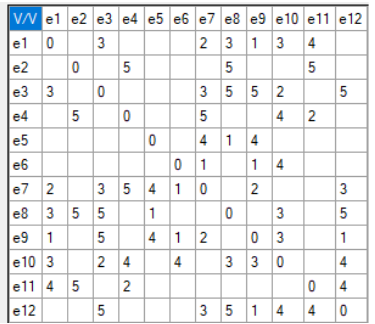
\includegraphics[width=\linewidth]{images/matrix.png}
        \caption{Матрица смежности}
        \label{fig:sub1}
    \end{subfigure}
    \hfill % Распорка для равномерного распределения
    \begin{subfigure}[b]{0.45\textwidth}
        
\includegraphics[width=\linewidth]{images/graph.png}
        \caption{Граф}
        \label{fig:sub2}
    \end{subfigure}
    %\caption{Общая подпись для двух картинок}
    \label{fig:main}
\end{figure}

\begin{table}[H]
    \centering
    \begin{tabular}{|l|l|l|l|l|l|l|l|l|l|l|l|l|}
    \hline
        v/v & $e_1$ & $e_2$ & $e_3$ & $e_4$ & $e_5$ & $e_6$ & $e_7$ & $e_8$ & $e_9$ & $e_{10}$ & $e_{11}$ & $e_{12}$ \\ \hline
        $e_1$ & 0 & 0 & 1 & 0 & 0 & 0 & 1 & 1 & 1 & 1 & 1 & 0 \\ \hline
        $e_2$ & 0 & 0 & 0 & 1 & 0 & 0 & 0 & 1 & 0 & 0 & 1 & 0 \\ \hline
        $e_3$ & 1 & 0 & 0 & 0 & 0 & 0 & 1 & 1 & 1 & 1 & 0 & 1 \\ \hline
        $e_4$ & 0 & 1 & 0 & 0 & 0 & 0 & 1 & 0 & 0 & 1 & 1 & 0 \\ \hline
        $e_5$ & 0 & 0 & 0 & 0 & 0 & 0 & 1 & 1 & 1 & 0 & 0 & 0 \\ \hline
        $e_6$ & 0 & 0 & 0 & 0 & 0 & 0 & 1 & 0 & 1 & 1 & 0 & 0 \\ \hline
        $e_7$ & 1 & 0 & 1 & 1 & 1 & 1 & 0 & 0 & 1 & 0 & 0 & 1 \\ \hline
        $e_8$ & 1 & 1 & 1 & 0 & 1 & 0 & 0 & 0 & 0 & 1 & 0 & 1 \\ \hline
        $e_9$ & 1 & 0 & 1 & 0 & 1 & 1 & 1 & 0 & 0 & 1 & 0 & 1 \\ \hline
        $e_{10}$ & 1 & 0 & 1 & 1 & 0 & 1 & 0 & 1 & 1 & 0 & 0 & 1 \\ \hline
        $e_{11}$ & 1 & 1 & 0 & 1 & 0 & 0 & 0 & 0 & 0 & 0 & 0 & 1 \\ \hline
        $e_{12}$ & 0 & 0 & 1 & 0 & 0 & 0 & 1 & 1 & 1 & 1 & 1 & 0 \\ \hline
    \end{tabular}
\end{table}

{ \large \centering \textbf{Нахождение гамильтонова цикла} \\ }
\noindent
Включаем в $S$ вершину $x_1$. $S = \{x_1\}$ \\
Возможная вершина: $x_{3}$. $S = \{x_{1},x_{3}\}$ \\
Возможная вершина: $x_{7}$. $S = \{x_{1},x_{3},x_{7}\}$ \\
Возможная вершина: $x_{4}$. $S = \{x_{1},x_{3},x_{7},x_{4}\}$ \\
Возможная вершина: $x_{2}$. $S = \{x_{1},x_{3},x_{7},x_{4},x_{2}\}$ \\
Возможная вершина: $x_{8}$. $S = \{x_{1},x_{3},x_{7},x_{4},x_{2},x_{8}\}$ \\
Возможная вершина: $x_{5}$. $S = \{x_{1},x_{3},x_{7},x_{4},x_{2},x_{8},x_{5}\}$ \\
Возможная вершина: $x_{9}$. $S = \{x_{1},x_{3},x_{7},x_{4},x_{2},x_{8},x_{5},x_{9}\}$ \\
Возможная вершина: $x_{6}$. $S = \{x_{1},x_{3},x_{7},x_{4},x_{2},x_{8},x_{5},x_{9},x_{6}\}$ \\
Возможная вершина: $x_{10}$. $S = \{x_{1},x_{3},x_{7},x_{4},x_{2},x_{8},x_{5},x_{9},x_{6},x_{10}\}$ \\
Возможная вершина: $x_{12}$. $S = \{x_{1},x_{3},x_{7},x_{4},x_{2},x_{8},x_{5},x_{9},x_{6},x_{10},x_{12}\}$ \\
Возможная вершина: $x_{11}$. $S = \{x_{1},x_{3},x_{7},x_{4},x_{2},x_{8},x_{5},x_{9},x_{6},x_{10},x_{12},x_{11}\}$ \\
Гамильтонов цикл найден. $S = \{x_{1},x_{3},x_{7},x_{4},x_{2},x_{8},x_{5},x_{9},x_{6},x_{10},x_{12},x_{11}\}$ \\

\begin{figure}[H]
    \centering
    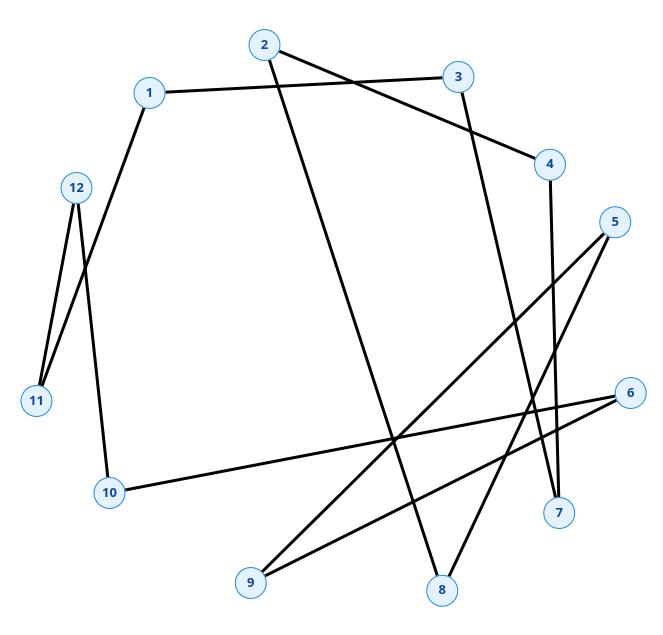
\includegraphics[width=0.7\linewidth]{images/4/gamiltonov.png}
    \caption*{Гамильтонов цикл графа}
\end{figure}

{ \large \centering \textbf{Матрица смежности с перенумерованными вершинами} \\ }
\begin{table}[H]
    \centering
    \begin{tabular}{|c|c|c|c|c|c|c|c|c|c|c|c|}
    \hline
        0 & 1 & 1 & 0 & 0 & 1 & 0 & 1 & 0 & 1 & 0 & 1 \\ \hline
        1 & 0 & 1 & 0 & 0 & 1 & 0 & 1 & 0 & 1 & 1 & 0 \\ \hline
        1 & 1 & 0 & 1 & 0 & 0 & 1 & 1 & 1 & 0 & 1 & 0 \\ \hline
        0 & 0 & 1 & 0 & 1 & 0 & 0 & 0 & 0 & 1 & 0 & 1 \\ \hline
        0 & 0 & 0 & 1 & 0 & 1 & 0 & 0 & 0 & 0 & 0 & 1 \\ \hline
        1 & 1 & 0 & 0 & 1 & 0 & 1 & 0 & 0 & 1 & 1 & 0 \\ \hline
        0 & 0 & 1 & 0 & 0 & 1 & 0 & 1 & 0 & 0 & 0 & 0 \\ \hline
        1 & 1 & 1 & 0 & 0 & 0 & 1 & 0 & 1 & 1 & 1 & 0 \\ \hline
        0 & 0 & 1 & 0 & 0 & 0 & 0 & 1 & 0 & 1 & 0 & 0 \\ \hline
        1 & 1 & 0 & 1 & 0 & 1 & 0 & 1 & 1 & 0 & 1 & 0 \\ \hline
        0 & 1 & 1 & 0 & 0 & 1 & 0 & 1 & 0 & 1 & 0 & 1 \\ \hline
        1 & 0 & 0 & 1 & 1 & 0 & 0 & 0 & 0 & 0 & 1 & 0 \\ \hline
    \end{tabular}
\end{table}
\noindent
до перенумерации $x_{1}$	$x_{2}$	$x_{3}$	$x_{4}$	$x_{5}$	$x_{6}$	$x_{7}$	$x_{8}$	$x_{9}$	$x_{10}$ $x_{11}$	$x_{12}$ \\
после перенумерации	$x_{1}$	$x_{3}$	$x_{7}$	$x_{4}$	$x_{2}$	$x_{8}$	$x_{5}$	$x_{9}$	$x_{6}$	$x_{10}$ $x_{12}$ $x_{11}$ \\
Перенумеруем вершины и расположим вершины гамильтонова цикла по окружности для удобства

\begin{figure}[H]
    \centering
    \begin{subfigure}[b]{0.45\textwidth}
        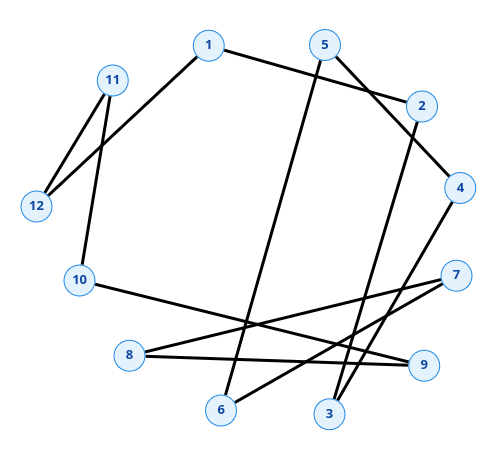
\includegraphics[width=\linewidth]{images/4/gamiltonov_renamed.png}
        \label{fig:sub1}
    \end{subfigure}
    \hfill % Распорка для равномерного распределения
    \begin{subfigure}[b]{0.45\textwidth}
        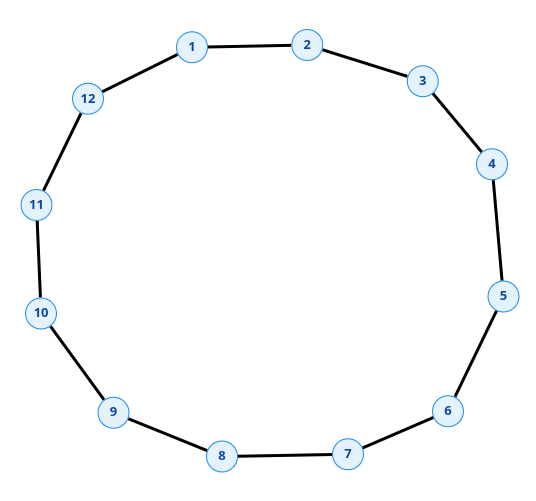
\includegraphics[width=\linewidth]{images/4/gamiltonov_circle.png}
        \label{fig:sub2}
    \end{subfigure}
    \caption*{Гамильтонов цикл после перенумерации}
    \label{fig:main}
\end{figure}

{ \large \centering \textbf{Построение графа пересечений $G'$} \\ }
\noindent
Определим $p_{211}$, для чего в матрице $R$ выделим подматрицу $R_{211}$. \\
Ребро $(x_{2}x_{11})$ пересекается с $(x_{1}x_{3}),(x_{1}x_{6}),(x_{1}x_{8}),(x_{1}x_{10})$ \\
Определим $p_{210}$, для чего в матрице $R$ выделим подматрицу $R_{210}$. \\
Ребро $(x_{2}x_{10})$ пересекается с $(x_{1}x_{3}),(x_{1}x_{6}),(x_{1}x_{8})$ \\
Определим $p_{28}$, для чего в матрице $R$ выделим подматрицу $R_{28}$. \\
Ребро $(x_{2}x_{8})$ пересекается с $(x_{1}x_{3}),(x_{1}x_{6})$ \\
Определим $p_{26}$, для чего в матрице $R$ выделим подматрицу $R_{26}$. \\
Ребро $(x_{2}x_{6})$ пересекается с $(x_{1}x_{3})$ \\
Определим $p_{311}$, для чего в матрице $R$ выделим подматрицу $R_{311}$. \\
Ребро $(x_{3}x_{11})$ пересекается с $(x_{1}x_{6}),(x_{1}x_{8}),(x_{1}x_{10}),(x_{2}x_{6}),(x_{2}x_{8}),(x_{2}x_{10})$ \\
Определим $p_{39}$, для чего в матрице $R$ выделим подматрицу $R_{39}$. \\
Ребро $(x_{3}x_{9})$ пересекается с $(x_{1}x_{6}),(x_{1}x_{8}),(x_{2}x_{6}),(x_{2}x_{8})$\\
Определим $p_{38}$, для чего в матрице $R$ выделим подматрицу $R_{38}$.\\
Ребро $(x_{3}x_{8})$ пересекается с $(x_{1}x_{6}),(x_{2}x_{6})$\\
Определим $p_{37}$, для чего в матрице $R$ выделим подматрицу $R_{37}$.\\
Ребро $(x_{3}x_{7})$ пересекается с $(x_{1}x_{6}),(x_{2}x_{6})$\\
Определим $p_{412}$, для чего в матрице $R$ выделим подматрицу $R_{412}$.\\
Ребро $(x_{4}x_{12})$ пересекается с $(x_{1}x_{6}),(x_{1}x_{8}),(x_{1}x_{10}),(x_{2}x_{6}),(x_{2}x_{8}), \\
(x_{2}x_{10}),(x_{2}x_{11}),(x_{3}x_{7}),(x_{3}x_{8}),(x_{3}x_{9}),(x_{3}x_{11})$\\
Определим $p_{410}$, для чего в матрице $R$ выделим подматрицу $R_{410}$.\\
Ребро $(x_{4}x_{10})$ пересекается с $(x_{1}x_{6}),(x_{1}x_{8}),(x_{2}x_{6}),(x_{2}x_{8}),(x_{3}x_{7}), \\
(x_{3}x_{8}),(x_{3}x_{9})$\\
Определим $p_{512}$, для чего в матрице $R$ выделим подматрицу $R_{512}$.\\
Ребро $(x_{5}x_{12})$ пересекается с $(x_{1}x_{6}),(x_{1}x_{8}),(x_{1}x_{10}),(x_{2}x_{6}),(x_{2}x_{8}),(x_{2}x_{10}),(x_{2}x_{11}), \\
(x_{3}x_{7}),(x_{3}x_{8}),(x_{3}x_{9}),(x_{3}x_{11}),(x_{4}x_{10})$\\
15 пересечений графа найдено, закончим поиск.\\

\begin{table}[H]
    \raggedleft
    \begin{tabular}{|c|c|c|c|c|c|c|c|c|c|c|c|c|c|c|c|}
    \hline
         & $p_{1\ 3}$ & $p_{2\ 11}$ & $p_{1\ 6}$ & $p_{1\ 8}$ & $p_{1\ 10}$ & $p_{2\ 10}$ & $p_{2\ 8}$ & $p_{2\ 6}$ & $p_{3\ 11}$ & $p_{3\ 9}$ & $p_{3\ 8}$ & $p_{3\ 7}$ & $p_{4\ 12}$ & $p_{4\ 10}$ & $p_{5\ 12}$ \\ \hline
        $p_{1\ 3}$ & 1 & 1 & 0 & 0 & 0 & 1 & 1 & 1 & 0 & 0 & 0 & 0 & 0 & 0 & 0 \\ \hline
        $p_{2\ 11}$ & 1 & 1 & 1 & 1 & 1 & 0 & 0 & 0 & 0 & 0 & 0 & 0 & 1 & 0 & 1 \\ \hline
        $p_{1\ 6}$ & 0 & 1 & 1 & 0 & 0 & 1 & 1 & 0 & 1 & 1 & 1 & 1 & 1 & 1 & 1 \\ \hline
        $p_{1\ 8}$ & 0 & 1 & 0 & 1 & 0 & 1 & 0 & 0 & 1 & 1 & 0 & 0 & 1 & 1 & 1 \\ \hline
        $p_{1\ 10}$ & 0 & 1 & 0 & 0 & 1 & 0 & 0 & 0 & 1 & 0 & 0 & 0 & 1 & 0 & 1 \\ \hline
        $p_{2\ 10}$ & 1 & 0 & 1 & 1 & 0 & 1 & 0 & 0 & 1 & 0 & 0 & 0 & 1 & 0 & 1 \\ \hline
        $p_{2\ 8}$ & 1 & 0 & 1 & 0 & 0 & 0 & 1 & 0 & 1 & 1 & 0 & 0 & 1 & 1 & 1 \\ \hline
        $p_{2\ 6}$ & 1 & 0 & 0 & 0 & 0 & 0 & 0 & 1 & 1 & 1 & 1 & 1 & 1 & 1 & 1 \\ \hline
        $p_{3\ 11}$ & 0 & 0 & 1 & 1 & 1 & 1 & 1 & 1 & 1 & 0 & 0 & 0 & 1 & 0 & 1 \\ \hline
        $p_{3\ 9}$ & 0 & 0 & 1 & 1 & 0 & 0 & 1 & 1 & 0 & 1 & 0 & 0 & 1 & 1 & 1 \\ \hline
        $p_{3\ 8}$ & 0 & 0 & 1 & 0 & 0 & 0 & 0 & 1 & 0 & 0 & 1 & 0 & 1 & 1 & 1 \\ \hline
        $p_{3\ 7}$ & 0 & 0 & 1 & 0 & 0 & 0 & 0 & 1 & 0 & 0 & 0 & 1 & 1 & 1 & 1 \\ \hline
        $p_{4\ 12}$ & 0 & 1 & 1 & 1 & 1 & 1 & 1 & 1 & 1 & 1 & 1 & 1 & 1 & 0 & 0 \\ \hline
        $p_{4\ 10}$ & 0 & 0 & 1 & 1 & 0 & 0 & 1 & 1 & 0 & 1 & 1 & 1 & 0 & 1 & 1 \\ \hline
        $p_{5\ 12}$ & 0 & 1 & 1 & 1 & 1 & 1 & 1 & 1 & 1 & 1 & 1 & 1 & 0 & 1 & 1 \\ \hline
    \end{tabular}
\end{table}

{ \large \centering \textbf{Построение семейства $\psi_G$} \\ }
\noindent
В 1 строке ищем первый нулевой элемент - $r_{1\ 3}$.\\
Записываем дизъюнкцию $M_{1\ 3} = r_{1}\lor r_{3} = 110001110000000 \lor 011001101111111 = 111001111111111$\\
В строке $M_{1\ 3}$ находим номера нулевых элементов, составляем список $J' = \{4, 5\}$.\\
Записываем дизъюнкцию $M_{1\ 3\ 4} = M_{1\ 3}\lor r_{4} = 111001111111111 \lor 010101001100111 = 111101111111111$\\
В строке $M_{1\ 3\ 4}$ находим номера нулевых элементов, составляем список $J' = \{5\}$.\\
Записываем дизъюнкцию $M_{1\ 3\ 4\ 5} = M_{1\ 3\ 4}\lor r_{5} = 111101111111111 \lor 010010001000101 = 111111111111111$\\
В строке $M_{1\ 3\ 4\ 5}$ все 1. Построено $\psi_{1} = \{u_{1\ 3},u_{1\ 6},u_{1\ 8},u_{1\ 10}\}$\\
Записываем дизъюнкцию $M_{1\ 3\ 5} = M_{1\ 3}\lor r_{5} = 111001111111111 \lor 010010001000101 = 111011111111111$\\
В строке $M_{1\ 3\ 5}$ остались незакрытые 0.\\
Записываем дизъюнкцию $M_{1\ 4} = r_{1}\lor r_{4} = 110001110000000 \lor 010101001100111 = 110101111100111$\\
В строке $M_{1\ 4}$ находим номера нулевых элементов, составляем список $J' = \{5, 11, 12\}$.\\
Записываем дизъюнкцию $M_{1\ 4\ 5} = M_{1\ 4}\lor r_{5} = 110101111100111 \lor 010010001000101 = 110111111100111$\\
В строке $M_{1\ 4\ 5}$ находим номера нулевых элементов, составляем список $J' = \{11, 12\}$.\\
Записываем дизъюнкцию $M_{1\ 4\ 5\ 11} = M_{1\ 4\ 5}\lor r_{11} = 110111111100111 \lor 001000010010111 = 111111111110111$\\
В строке $M_{1\ 4\ 5\ 11}$ находим номера нулевых элементов, составляем список $J' = \{12\}$.\\
Записываем дизъюнкцию $M_{1\ 4\ 5\ 11\ 12} = M_{1\ 4\ 5\ 11}\lor r_{12} = 111111111110111 \lor 001000010001111 = 111111111111111$\\
В строке $M_{1\ 4\ 5\ 11\ 12}$ все 1. Построено $\psi_{2} = \{u_{1\ 3},u_{1\ 8},u_{1\ 10},u_{3\ 8},u_{3\ 7}\}$\\
Записываем дизъюнкцию $M_{1\ 4\ 5\ 12} = M_{1\ 4\ 5}\lor r_{12} = 110111111100111 \lor 001000010001111 = 111111111101111$\\
В строке $M_{1\ 4\ 5\ 12}$ остались незакрытые 0.\\
Записываем дизъюнкцию $M_{1\ 4\ 11} = M_{1\ 4}\lor r_{11} = 110101111100111 \lor 001000010010111 = 111101111110111$\\
В строке $M_{1\ 4\ 11}$ находим номера нулевых элементов, составляем список $J' = \{12\}$.\\
Строка 12 не закроет ноль на 5 позиции.\\
Записываем дизъюнкцию $M_{1\ 4\ 12} = M_{1\ 4}\lor r_{12} = 110101111100111 \lor 001000010001111 = 111101111101111$\\
В строке $M_{1\ 4\ 12}$ остались незакрытые 0.\\
Записываем дизъюнкцию $M_{1\ 5} = r_{1}\lor r_{5} = 110001110000000 \lor 010010001000101 = 110011111000101$\\
В строке $M_{1\ 5}$ находим номера нулевых элементов, составляем список $J' = \{10, 11, 12, 14\}$.\\
Записываем дизъюнкцию $M_{1\ 5\ 10} = M_{1\ 5}\lor r_{10} = 110011111000101 \lor 001100110100111 = 111111111100111$\\
В строке $M_{1\ 5\ 10}$ находим номера нулевых элементов, составляем список $J' = \{11, 12\}$.\\
Записываем дизъюнкцию $M_{1\ 5\ 10\ 11} = M_{1\ 5\ 10}\lor r_{11} = 111111111100111 \lor 001000010010111 = 111111111110111$\\
В строке $M_{1\ 5\ 10\ 11}$ находим номера нулевых элементов, составляем список $J' = \{12\}$.\\
Записываем дизъюнкцию $M_{1\ 5\ 10\ 11\ 12} = M_{1\ 5\ 10\ 11}\lor r_{12} = 111111111110111 \lor 001000010001111 = 111111111111111$\\
В строке $M_{1\ 5\ 10\ 11\ 12}$ все 1. Построено $\psi_{3} = \{u_{1\ 3},u_{1\ 10},u_{3\ 9},u_{3\ 8},u_{3\ 7}\}$\\
Записываем дизъюнкцию $M_{1\ 5\ 10\ 12} = M_{1\ 5\ 10}\lor r_{12} = 111111111100111 \lor 001000010001111 = 111111111101111$\\
В строке $M_{1\ 5\ 10\ 12}$ остались незакрытые 0.\\
Записываем дизъюнкцию $M_{1\ 5\ 11} = M_{1\ 5}\lor r_{11} = 110011111000101 \lor 001000010010111 = 111011111010111$\\
В строке $M_{1\ 5\ 11}$ находим номера нулевых элементов, составляем список $J' = \{12\}$.\\
Строка 12 не закроет нули на позициях 4, 10\\
Записываем дизъюнкцию $M_{1\ 5\ 12} = M_{1\ 5}\lor r_{12} = 110011111000101 \lor 001000010001111 = 111011111001111$\\
В строке $M_{1\ 5\ 12}$ остались незакрытые 0.\\
Записываем дизъюнкцию $M_{1\ 5\ 14} = M_{1\ 5}\lor r_{14} = 110011111000101 \lor 001100110111011 = 111111111111111$\\
В строке $M_{1\ 5\ 14}$ все 1. Построено $\psi_{4} = \{u_{1\ 3},u_{1\ 10},u_{4\ 10}\}$\\
Записываем дизъюнкцию $M_{1\ 9} = r_{1}\lor r_{9} = 110001110000000 \lor 001111111000101 = 111111111000101$\\
В строке $M_{1\ 9}$ находим номера нулевых элементов, составляем список $J' = \{10, 11, 12, 14\}$.\\
Записываем дизъюнкцию $M_{1\ 9\ 10} = M_{1\ 9}\lor r_{10} = 111111111000101 \lor 001100110100111 = 111111111100111$\\
В строке $M_{1\ 9\ 10}$ находим номера нулевых элементов, составляем список $J' = \{11, 12\}$.\\
Записываем дизъюнкцию $M_{1\ 9\ 10\ 11} = M_{1\ 9\ 10}\lor r_{11} = 111111111100111 \lor 001000010010111 = 111111111110111$\\
В строке $M_{1\ 9\ 10\ 11}$ находим номера нулевых элементов, составляем список $J' = \{12\}$.\\
Записываем дизъюнкцию $M_{1\ 9\ 10\ 11\ 12} = M_{1\ 9\ 10\ 11}\lor r_{12} = 111111111110111 \lor 001000010001111 = 111111111111111$\\
В строке $M_{1\ 9\ 10\ 11\ 12}$ все 1. Построено $\psi_{5} = \{u_{1\ 3},u_{3\ 11},u_{3\ 9},u_{3\ 8},u_{3\ 7}\}$\\
Записываем дизъюнкцию $M_{1\ 9\ 10\ 12} = M_{1\ 9\ 10}\lor r_{12} = 111111111100111 \lor 001000010001111 = 111111111101111$\\
В строке $M_{1\ 9\ 10\ 12}$ остались незакрытые 0.\\
Записываем дизъюнкцию $M_{1\ 9\ 11} = M_{1\ 9}\lor r_{11} = 111111111000101 \lor 001000010010111 = 111111111010111$\\
В строке $M_{1\ 9\ 11}$ находим номера нулевых элементов, составляем список $J' = \{12\}$.\\
Строка 12 не закроет ноль на 10 позиции.\\
Записываем дизъюнкцию $M_{1\ 9\ 12} = M_{1\ 9}\lor r_{12} = 111111111000101 \lor 001000010001111 = 111111111001111$\\
В строке $M_{1\ 9\ 12}$ остались незакрытые 0.\\
Записываем дизъюнкцию $M_{1\ 9\ 14} = M_{1\ 9}\lor r_{14} = 111111111000101 \lor 001100110111011 = 111111111111111$\\
В строке $M_{1\ 9\ 14}$ все 1. Построено $\psi_{6} = \{u_{1\ 3},u_{3\ 11},u_{4\ 10}\}$\\
Записываем дизъюнкцию $M_{1\ 10} = r_{1}\lor r_{10} = 110001110000000 \lor 001100110100111 = 111101110100111$\\
В строке $M_{1\ 10}$ находим номера нулевых элементов, составляем список $J' = \{11, 12\}$.\\
Строки 11, 12 не закроют нули на позициях 5, 9\\
Записываем дизъюнкцию $M_{1\ 11} = r_{1}\lor r_{11} = 110001110000000 \lor 001000010010111 = 111001110010111$\\
В строке $M_{1\ 11}$ находим номера нулевых элементов, составляем список $J' = \{12\}$.\\
Строка 12 не закроет нули на позициях 4, 5, 9, 10\\
Записываем дизъюнкцию $M_{1\ 12} = r_{1}\lor r_{12} = 110001110000000 \lor 001000010001111 = 111001110001111$\\
В строке $M_{1\ 12}$ остались незакрытые 0.\\
Записываем дизъюнкцию $M_{1\ 13} = r_{1}\lor r_{13} = 110001110000000 \lor 011111111111100 = 111111111111100$\\
В строке $M_{1\ 13}$ находим номера нулевых элементов, составляем список $J' = \{14, 15\}$.\\
Записываем дизъюнкцию $M_{1\ 13\ 14} = M_{1\ 13}\lor r_{14} = 111111111111100 \lor 001100110111011 = 111111111111111$\\
В строке $M_{1\ 13\ 14}$ все 1. Построено $\psi_{7} = \{u_{1\ 3},u_{4\ 12},u_{4\ 10}\}$\\
Записываем дизъюнкцию $M_{1\ 13\ 15} = M_{1\ 13}\lor r_{15} = 111111111111100 \lor 011111111111011 = 111111111111111$\\
В строке $M_{1\ 13\ 15}$ все 1. Построено $\psi_{8} = \{u_{1\ 3},u_{4\ 12},u_{5\ 12}\}$\\
Записываем дизъюнкцию $M_{1\ 14} = r_{1}\lor r_{14} = 110001110000000 \lor 001100110111011 = 111101110111011$\\
В строке $M_{1\ 14}$ остались незакрытые 0.\\
Записываем дизъюнкцию $M_{1\ 15} = r_{1}\lor r_{15} = 110001110000000 \lor 011111111111011 = 111111111111011$\\
В строке $M_{1\ 15}$ остались незакрытые 0.\\

\noindent
В 2 строке ищем первый нулевой элемент - $r_{2\ 6}$.\\
Записываем дизъюнкцию $M_{2\ 6} = r_{2}\lor r_{6} = 111110000000101 \lor 101101001000101 = 111111001000101$\\
В строке $M_{2\ 6}$ находим номера нулевых элементов, составляем список $J' = \{7, 8, 10, 11, 12, 14\}$.\\
Записываем дизъюнкцию $M_{2\ 6\ 7} = M_{2\ 6}\lor r_{7} = 111111001000101 \lor 101000101100111 = 111111101100111$\\
В строке $M_{2\ 6\ 7}$ находим номера нулевых элементов, составляем список $J' = \{8, 11, 12\}$.\\
Записываем дизъюнкцию $M_{2\ 6\ 7\ 8} = M_{2\ 6\ 7}\lor r_{8} = 111111101100111 \lor 100000011111111 = 111111111111111$\\
В строке $M_{2\ 6\ 7\ 8}$ все 1. Построено $\psi_{9} = \{u_{2\ 11},u_{2\ 10},u_{2\ 8},u_{2\ 6}\}$\\
Записываем дизъюнкцию $M_{2\ 6\ 7\ 11} = M_{2\ 6\ 7}\lor r_{11} = 111111101100111 \lor 001000010010111 = 111111111110111$\\
В строке $M_{2\ 6\ 7\ 11}$ находим номера нулевых элементов, составляем список $J' = \{12\}$.\\
Записываем дизъюнкцию $M_{2\ 6\ 7\ 11\ 12} = M_{2\ 6\ 7\ 11}\lor r_{12} = 111111111110111 \lor 001000010001111 = 111111111111111$\\
В строке $M_{2\ 6\ 7\ 11\ 12}$ все 1. Построено $\psi_{10} = \{u_{2\ 11},u_{2\ 10},u_{2\ 8},u_{3\ 8},u_{3\ 7}\}$\\
Записываем дизъюнкцию $M_{2\ 6\ 7\ 12} = M_{2\ 6\ 7}\lor r_{12} = 111111101100111 \lor 001000010001111 = 111111111101111$\\
В строке $M_{2\ 6\ 7\ 12}$ остались незакрытые 0.\\
Записываем дизъюнкцию $M_{2\ 6\ 8} = M_{2\ 6}\lor r_{8} = 111111001000101 \lor 100000011111111 = 111111011111111$\\
В строке $M_{2\ 6\ 8}$ остались незакрытые 0.\\
Записываем дизъюнкцию $M_{2\ 6\ 10} = M_{2\ 6}\lor r_{10} = 111111001000101 \lor 001100110100111 = 111111111100111$\\
В строке $M_{2\ 6\ 10}$ находим номера нулевых элементов, составляем список $J' = \{11, 12\}$.\\
Записываем дизъюнкцию $M_{2\ 6\ 10\ 11} = M_{2\ 6\ 10}\lor r_{11} = 111111111100111 \lor 001000010010111 = 111111111110111$\\
В строке $M_{2\ 6\ 10\ 11}$ находим номера нулевых элементов, составляем список $J' = \{12\}$.\\
Записываем дизъюнкцию $M_{2\ 6\ 10\ 11\ 12} = M_{2\ 6\ 10\ 11}\lor r_{12} = 111111111110111 \lor 001000010001111 = 111111111111111$\\
В строке $M_{2\ 6\ 10\ 11\ 12}$ все 1. Построено $\psi_{11} = \{u_{2\ 11},u_{2\ 10},u_{3\ 9},u_{3\ 8},u_{3\ 7}\}$\\
Записываем дизъюнкцию $M_{2\ 6\ 10\ 12} = M_{2\ 6\ 10}\lor r_{12} = 111111111100111 \lor 001000010001111 = 111111111101111$\\
В строке $M_{2\ 6\ 10\ 12}$ остались незакрытые 0.\\
Записываем дизъюнкцию $M_{2\ 6\ 11} = M_{2\ 6}\lor r_{11} = 111111001000101 \lor 001000010010111 = 111111011010111$\\
В строке $M_{2\ 6\ 11}$ находим номера нулевых элементов, составляем список $J' = \{12\}$.\\
Строка 12 не закроет нули на позициях 7, 10\\
Записываем дизъюнкцию $M_{2\ 6\ 12} = M_{2\ 6}\lor r_{12} = 111111001000101 \lor 001000010001111 = 111111011001111$\\
В строке $M_{2\ 6\ 12}$ остались незакрытые 0.\\
Записываем дизъюнкцию $M_{2\ 6\ 14} = M_{2\ 6}\lor r_{14} = 111111001000101 \lor 001100110111011 = 111111111111111$\\
В строке $M_{2\ 6\ 14}$ все 1. Построено $\psi_{12} = \{u_{2\ 11},u_{2\ 10},u_{4\ 10}\}$\\
Записываем дизъюнкцию $M_{2\ 7} = r_{2}\lor r_{7} = 111110000000101 \lor 101000101100111 = 111110101100111$\\
В строке $M_{2\ 7}$ находим номера нулевых элементов, составляем список $J' = \{8, 11, 12\}$.\\
Строки 8, 11, 12 не закроют ноль на 6 позиции.\\
Записываем дизъюнкцию $M_{2\ 8} = r_{2}\lor r_{8} = 111110000000101 \lor 100000011111111 = 111110011111111$\\
В строке $M_{2\ 8}$ остались незакрытые 0.\\
Записываем дизъюнкцию $M_{2\ 9} = r_{2}\lor r_{9} = 111110000000101 \lor 001111111000101 = 111111111000101$\\
В строке $M_{2\ 9}$ находим номера нулевых элементов, составляем список $J' = \{10, 11, 12, 14\}$.\\
Записываем дизъюнкцию $M_{2\ 9\ 10} = M_{2\ 9}\lor r_{10} = 111111111000101 \lor 001100110100111 = 111111111100111$\\
В строке $M_{2\ 9\ 10}$ находим номера нулевых элементов, составляем список $J' = \{11, 12\}$.\\
Записываем дизъюнкцию $M_{2\ 9\ 10\ 11} = M_{2\ 9\ 10}\lor r_{11} = 111111111100111 \lor 001000010010111 = 111111111110111$\\
В строке $M_{2\ 9\ 10\ 11}$ находим номера нулевых элементов, составляем список $J' = \{12\}$.\\
Записываем дизъюнкцию $M_{2\ 9\ 10\ 11\ 12} = M_{2\ 9\ 10\ 11}\lor r_{12} = 111111111110111 \lor 001000010001111 = 111111111111111$\\
В строке $M_{2\ 9\ 10\ 11\ 12}$ все 1. Построено $\psi_{13} = \{u_{2\ 11},u_{3\ 11},u_{3\ 9},u_{3\ 8},u_{3\ 7}\}$\\
Записываем дизъюнкцию $M_{2\ 9\ 10\ 12} = M_{2\ 9\ 10}\lor r_{12} = 111111111100111 \lor 001000010001111 = 111111111101111$\\
В строке $M_{2\ 9\ 10\ 12}$ остались незакрытые 0.\\
Записываем дизъюнкцию $M_{2\ 9\ 11} = M_{2\ 9}\lor r_{11} = 111111111000101 \lor 001000010010111 = 111111111010111$\\
В строке $M_{2\ 9\ 11}$ находим номера нулевых элементов, составляем список $J' = \{12\}$.\\
Строка 12 не закроет ноль на 10 позиции.\\
Записываем дизъюнкцию $M_{2\ 9\ 12} = M_{2\ 9}\lor r_{12} = 111111111000101 \lor 001000010001111 = 111111111001111$\\
В строке $M_{2\ 9\ 12}$ остались незакрытые 0.\\
Записываем дизъюнкцию $M_{2\ 9\ 14} = M_{2\ 9}\lor r_{14} = 111111111000101 \lor 001100110111011 = 111111111111111$\\
В строке $M_{2\ 9\ 14}$ все 1. Построено $\psi_{14} = \{u_{2\ 11},u_{3\ 11},u_{4\ 10}\}$\\
Записываем дизъюнкцию $M_{2\ 10} = r_{2}\lor r_{10} = 111110000000101 \lor 001100110100111 = 111110110100111$\\
В строке $M_{2\ 10}$ находим номера нулевых элементов, составляем список $J' = \{11, 12\}$.\\
Строки 11, 12 не закроют нули на позициях 6, 9\\
Записываем дизъюнкцию $M_{2\ 11} = r_{2}\lor r_{11} = 111110000000101 \lor 001000010010111 = 111110010010111$\\
В строке $M_{2\ 11}$ находим номера нулевых элементов, составляем список $J' = \{12\}$.\\
Строка 12 не закроет нули на позициях 6, 7, 9, 10\\
Записываем дизъюнкцию $M_{2\ 12} = r_{2}\lor r_{12} = 111110000000101 \lor 001000010001111 = 111110010001111$\\
В строке $M_{2\ 12}$ остались незакрытые 0.\\
Записываем дизъюнкцию $M_{2\ 14} = r_{2}\lor r_{14} = 111110000000101 \lor 001100110111011 = 111110110111111$\\
В строке $M_{2\ 14}$ остались незакрытые 0.\\

\noindent
В 3 строке ищем первый нулевой элемент - $r_{3\ 4}$.\\
Записываем дизъюнкцию $M_{3\ 4} = r_{3}\lor r_{4} = 011001101111111 \lor 010101001100111 = 011101101111111$\\
В строке $M_{3\ 4}$ находим номера нулевых элементов, составляем список $J' = \{5, 8\}$.\\
Записываем дизъюнкцию $M_{3\ 4\ 5} = M_{3\ 4}\lor r_{5} = 011101101111111 \lor 010010001000101 = 011111101111111$\\
В строке $M_{3\ 4\ 5}$ находим номера нулевых элементов, составляем список $J' = \{8\}$.\\
Записываем дизъюнкцию $M_{3\ 4\ 5\ 8} = M_{3\ 4\ 5}\lor r_{8} = 011111101111111 \lor 100000011111111 = 111111111111111$\\
В строке $M_{3\ 4\ 5\ 8}$ все 1. Построено $\psi_{15} = \{u_{1\ 6},u_{1\ 8},u_{1\ 10},u_{2\ 6}\}$\\
Записываем дизъюнкцию $M_{3\ 4\ 8} = M_{3\ 4}\lor r_{8} = 011101101111111 \lor 100000011111111 = 111101111111111$\\
В строке $M_{3\ 4\ 8}$ остались незакрытые 0.\\
Записываем дизъюнкцию $M_{3\ 5} = r_{3}\lor r_{5} = 011001101111111 \lor 010010001000101 = 011011101111111$\\
В строке $M_{3\ 5}$ находим номера нулевых элементов, составляем список $J' = \{8\}$.\\
Строка 8 не закроет ноль на 4 позиции.\\
Записываем дизъюнкцию $M_{3\ 8} = r_{3}\lor r_{8} = 011001101111111 \lor 100000011111111 = 111001111111111$\\
В строке $M_{3\ 8}$ остались незакрытые 0.\\


\noindent
В 4 строке ищем первый нулевой элемент - $r_{4\ 5}$.\\
Записываем дизъюнкцию $M_{4\ 5} = r_{4}\lor r_{5} = 010101001100111 \lor 010010001000101 = 010111001100111$\\
В строке $M_{4\ 5}$ находим номера нулевых элементов, составляем список $J' = \{7, 8, 11, 12\}$.\\
Записываем дизъюнкцию $M_{4\ 5\ 7} = M_{4\ 5}\lor r_{7} = 010111001100111 \lor 101000101100111 = 111111101100111$\\
В строке $M_{4\ 5\ 7}$ находим номера нулевых элементов, составляем список $J' = \{8, 11, 12\}$.\\
Записываем дизъюнкцию $M_{4\ 5\ 7\ 8} = M_{4\ 5\ 7}\lor r_{8} = 111111101100111 \lor 100000011111111 = 111111111111111$\\
В строке $M_{4\ 5\ 7\ 8}$ все 1. Построено $\psi_{16} = \{u_{1\ 8},u_{1\ 10},u_{2\ 8},u_{2\ 6}\}$\\
Записываем дизъюнкцию $M_{4\ 5\ 7\ 11} = M_{4\ 5\ 7}\lor r_{11} = 111111101100111 \lor 001000010010111 = 111111111110111$\\
В строке $M_{4\ 5\ 7\ 11}$ находим номера нулевых элементов, составляем список $J' = \{12\}$.\\
Записываем дизъюнкцию $M_{4\ 5\ 7\ 11\ 12} = M_{4\ 5\ 7\ 11}\lor r_{12} = 111111111110111 \lor 001000010001111 = 111111111111111$\\
В строке $M_{4\ 5\ 7\ 11\ 12}$ все 1. Построено $\psi_{17} = \{u_{1\ 8},u_{1\ 10},u_{2\ 8},u_{3\ 8},u_{3\ 7}\}$\\
Записываем дизъюнкцию $M_{4\ 5\ 7\ 12} = M_{4\ 5\ 7}\lor r_{12} = 111111101100111 \lor 001000010001111 = 111111111101111$\\
В строке $M_{4\ 5\ 7\ 12}$ остались незакрытые 0.\\
Записываем дизъюнкцию $M_{4\ 5\ 8} = M_{4\ 5}\lor r_{8} = 010111001100111 \lor 100000011111111 = 110111011111111$\\
В строке $M_{4\ 5\ 8}$ остались незакрытые 0.\\
Записываем дизъюнкцию $M_{4\ 5\ 11} = M_{4\ 5}\lor r_{11} = 010111001100111 \lor 001000010010111 = 011111011110111$\\
В строке $M_{4\ 5\ 11}$ находим номера нулевых элементов, составляем список $J' = \{12\}$.\\
Строка 12 не закроет нули на позициях 1, 7\\
Записываем дизъюнкцию $M_{4\ 5\ 12} = M_{4\ 5}\lor r_{12} = 010111001100111 \lor 001000010001111 = 011111011101111$\\
В строке $M_{4\ 5\ 12}$ остались незакрытые 0.\\
Записываем дизъюнкцию $M_{4\ 7} = r_{4}\lor r_{7} = 010101001100111 \lor 101000101100111 = 111101101100111$\\
В строке $M_{4\ 7}$ находим номера нулевых элементов, составляем список $J' = \{8, 11, 12\}$.\\
Строки 8, 11, 12 не закроют ноль на 5 позиции.\\
Записываем дизъюнкцию $M_{4\ 8} = r_{4}\lor r_{8} = 010101001100111 \lor 100000011111111 = 110101011111111$\\
В строке $M_{4\ 8}$ остались незакрытые 0.\\
Записываем дизъюнкцию $M_{4\ 11} = r_{4}\lor r_{11} = 010101001100111 \lor 001000010010111 = 011101011110111$\\
В строке $M_{4\ 11}$ находим номера нулевых элементов, составляем список $J' = \{12\}$.\\
Строка 12 не закроет нули на позициях 1, 5, 7\\
Записываем дизъюнкцию $M_{4\ 12} = r_{4}\lor r_{12} = 010101001100111 \lor 001000010001111 = 011101011101111$\\
В строке $M_{4\ 12}$ остались незакрытые 0.\\

\noindent
В 5 строке ищем первый нулевой элемент - $r_{5\ 6}$.\\
Записываем дизъюнкцию $M_{5\ 6} = r_{5}\lor r_{6} = 010010001000101 \lor 101101001000101 = 111111001000101$\\
В строке $M_{5\ 6}$ находим номера нулевых элементов, составляем список $J' = \{7, 8, 10, 11, 12, 14\}$.\\
Записываем дизъюнкцию $M_{5\ 6\ 7} = M_{5\ 6}\lor r_{7} = 111111001000101 \lor 101000101100111 = 111111101100111$\\
В строке $M_{5\ 6\ 7}$ находим номера нулевых элементов, составляем список $J' = \{8, 11, 12\}$.\\
Записываем дизъюнкцию $M_{5\ 6\ 7\ 8} = M_{5\ 6\ 7}\lor r_{8} = 111111101100111 \lor 100000011111111 = 111111111111111$\\
В строке $M_{5\ 6\ 7\ 8}$ все 1. Построено $\psi_{18} = \{u_{1\ 10},u_{2\ 10},u_{2\ 8},u_{2\ 6}\}$\\
Записываем дизъюнкцию $M_{5\ 6\ 7\ 11} = M_{5\ 6\ 7}\lor r_{11} = 111111101100111 \lor 001000010010111 = 111111111110111$\\
В строке $M_{5\ 6\ 7\ 11}$ находим номера нулевых элементов, составляем список $J' = \{12\}$.\\
Записываем дизъюнкцию $M_{5\ 6\ 7\ 11\ 12} = M_{5\ 6\ 7\ 11}\lor r_{12} = 111111111110111 \lor 001000010001111 = 111111111111111$\\
В строке $M_{5\ 6\ 7\ 11\ 12}$ все 1. Построено $\psi_{19} = \{u_{1\ 10},u_{2\ 10},u_{2\ 8},u_{3\ 8},u_{3\ 7}\}$\\
Записываем дизъюнкцию $M_{5\ 6\ 7\ 12} = M_{5\ 6\ 7}\lor r_{12} = 111111101100111 \lor 001000010001111 = 111111111101111$\\
В строке $M_{5\ 6\ 7\ 12}$ остались незакрытые 0.\\
Записываем дизъюнкцию $M_{5\ 6\ 8} = M_{5\ 6}\lor r_{8} = 111111001000101 \lor 100000011111111 = 111111011111111$\\
В строке $M_{5\ 6\ 8}$ остались незакрытые 0.\\
Записываем дизъюнкцию $M_{5\ 6\ 10} = M_{5\ 6}\lor r_{10} = 111111001000101 \lor 001100110100111 = 111111111100111$\\
В строке $M_{5\ 6\ 10}$ находим номера нулевых элементов, составляем список $J' = \{11, 12\}$.\\
Записываем дизъюнкцию $M_{5\ 6\ 10\ 11} = M_{5\ 6\ 10}\lor r_{11} = 111111111100111 \lor 001000010010111 = 111111111110111$\\
В строке $M_{5\ 6\ 10\ 11}$ находим номера нулевых элементов, составляем список $J' = \{12\}$.\\
Записываем дизъюнкцию $M_{5\ 6\ 10\ 11\ 12} = M_{5\ 6\ 10\ 11}\lor r_{12} = 111111111110111 \lor 001000010001111 = 111111111111111$\\
В строке $M_{5\ 6\ 10\ 11\ 12}$ все 1. Построено $\psi_{20} = \{u_{1\ 10},u_{2\ 10},u_{3\ 9},u_{3\ 8},u_{3\ 7}\}$\\
Записываем дизъюнкцию $M_{5\ 6\ 10\ 12} = M_{5\ 6\ 10}\lor r_{12} = 111111111100111 \lor 001000010001111 = 111111111101111$\\
В строке $M_{5\ 6\ 10\ 12}$ остались незакрытые 0.\\
Записываем дизъюнкцию $M_{5\ 6\ 11} = M_{5\ 6}\lor r_{11} = 111111001000101 \lor 001000010010111 = 111111011010111$\\
В строке $M_{5\ 6\ 11}$ находим номера нулевых элементов, составляем список $J' = \{12\}$.\\
Строка 12 не закроет нули на позициях 7, 10\\
Записываем дизъюнкцию $M_{5\ 6\ 12} = M_{5\ 6}\lor r_{12} = 111111001000101 \lor 001000010001111 = 111111011001111$\\
В строке $M_{5\ 6\ 12}$ остались незакрытые 0.\\
Записываем дизъюнкцию $M_{5\ 6\ 14} = M_{5\ 6}\lor r_{14} = 111111001000101 \lor 001100110111011 = 111111111111111$\\
В строке $M_{5\ 6\ 14}$ все 1. Построено $\psi_{21} = \{u_{1\ 10},u_{2\ 10},u_{4\ 10}\}$\\
Записываем дизъюнкцию $M_{5\ 7} = r_{5}\lor r_{7} = 010010001000101 \lor 101000101100111 = 111010101100111$\\
В строке $M_{5\ 7}$ находим номера нулевых элементов, составляем список $J' = \{8, 11, 12\}$.\\
Строки 8, 11, 12 не закроют нули на позициях 4, 6\\
Записываем дизъюнкцию $M_{5\ 8} = r_{5}\lor r_{8} = 010010001000101 \lor 100000011111111 = 110010011111111$\\
В строке $M_{5\ 8}$ остались незакрытые 0.\\
Записываем дизъюнкцию $M_{5\ 10} = r_{5}\lor r_{10} = 010010001000101 \lor 001100110100111 = 011110111100111$\\
В строке $M_{5\ 10}$ находим номера нулевых элементов, составляем список $J' = \{11, 12\}$.\\
Строки 11, 12 не закроют нули на позициях 1, 6\\
Записываем дизъюнкцию $M_{5\ 11} = r_{5}\lor r_{11} = 010010001000101 \lor 001000010010111 = 011010011010111$\\
В строке $M_{5\ 11}$ находим номера нулевых элементов, составляем список $J' = \{12\}$.\\
Строка 12 не закроет нули на позициях 1, 4, 6, 7, 10\\
Записываем дизъюнкцию $M_{5\ 12} = r_{5}\lor r_{12} = 010010001000101 \lor 001000010001111 = 011010011001111$\\
В строке $M_{5\ 12}$ остались незакрытые 0.\\
Записываем дизъюнкцию $M_{5\ 14} = r_{5}\lor r_{14} = 010010001000101 \lor 001100110111011 = 011110111111111$\\
В строке $M_{5\ 14}$ остались незакрытые 0.\\

\noindent
В 6 строке ищем первый нулевой элемент - $r_{6\ 7}$.\\
Записываем дизъюнкцию $M_{6\ 7} = r_{6}\lor r_{7} = 101101001000101 \lor 101000101100111 = 101101101100111$\\
В строке $M_{6\ 7}$ находим номера нулевых элементов, составляем список $J' = \{8, 11, 12\}$.\\
Строки 8, 11, 12 не закроют нули на позициях 2, 5\\
Записываем дизъюнкцию $M_{6\ 8} = r_{6}\lor r_{8} = 101101001000101 \lor 100000011111111 = 101101011111111$\\
В строке $M_{6\ 8}$ остались незакрытые 0.\\
Записываем дизъюнкцию $M_{6\ 10} = r_{6}\lor r_{10} = 101101001000101 \lor 001100110100111 = 101101111100111$\\
В строке $M_{6\ 10}$ находим номера нулевых элементов, составляем список $J' = \{11, 12\}$.\\
Строки 11, 12 не закроют нули на позициях 2, 5\\
Записываем дизъюнкцию $M_{6\ 11} = r_{6}\lor r_{11} = 101101001000101 \lor 001000010010111 = 101101011010111$\\
В строке $M_{6\ 11}$ находим номера нулевых элементов, составляем список $J' = \{12\}$.\\
Строка 12 не закроет нули на позициях 2, 5, 7, 10\\
Записываем дизъюнкцию $M_{6\ 12} = r_{6}\lor r_{12} = 101101001000101 \lor 001000010001111 = 101101011001111$\\
В строке $M_{6\ 12}$ остались незакрытые 0.\\
Записываем дизъюнкцию $M_{6\ 14} = r_{6}\lor r_{14} = 101101001000101 \lor 001100110111011 = 101101111111111$\\
В строке $M_{6\ 14}$ остались незакрытые 0.\\

\noindent
В 7 строке ищем первый нулевой элемент - $r_{7\ 8}$.\\
Записываем дизъюнкцию $M_{7\ 8} = r_{7}\lor r_{8} = 101000101100111 \lor 100000011111111 = 101000111111111$\\
В строке $M_{7\ 8}$ остались незакрытые 0.\\
Записываем дизъюнкцию $M_{7\ 11} = r_{7}\lor r_{11} = 101000101100111 \lor 001000010010111 = 101000111110111$\\
В строке $M_{7\ 11}$ находим номера нулевых элементов, составляем список $J' = \{12\}$.\\
Строка 12 не закроет нули на позициях 2, 4, 5, 6\\
Записываем дизъюнкцию $M_{7\ 12} = r_{7}\lor r_{12} = 101000101100111 \lor 001000010001111 = 101000111101111$\\
В строке $M_{7\ 12}$ остались незакрытые 0.\\

\noindent
$\psi_22 = \{8\}$ \\
Из матрицы $R(G')$ видно, что строки с номерами j > 8 не смогут закрыть ноль в позиции 1. \\

\noindent
Семейство максимальных внутренне устойчивых множеств $\psi_G$ построено. Это:\\
$\psi_{1} = \{u_{1\ 3},u_{1\ 6},u_{1\ 8},u_{1\ 10}\}$\\
$\psi_{2} = \{u_{1\ 3},u_{1\ 8},u_{1\ 10},u_{3\ 8},u_{3\ 7}\}$\\
$\psi_{3} = \{u_{1\ 3},u_{1\ 10},u_{3\ 9},u_{3\ 8},u_{3\ 7}\}$\\
$\psi_{4} = \{u_{1\ 3},u_{1\ 10},u_{4\ 10}\}$\\
$\psi_{5} = \{u_{1\ 3},u_{3\ 11},u_{3\ 9},u_{3\ 8},u_{3\ 7}\}$\\
$\psi_{6} = \{u_{1\ 3},u_{3\ 11},u_{4\ 10}\}$\\
$\psi_{7} = \{u_{1\ 3},u_{4\ 12},u_{4\ 10}\}$\\
$\psi_{8} = \{u_{1\ 3},u_{4\ 12},u_{5\ 12}\}$\\
$\psi_{9} = \{u_{2\ 11},u_{2\ 10},u_{2\ 8},u_{2\ 6}\}$\\
$\psi_{10} = \{u_{2\ 11},u_{2\ 10},u_{2\ 8},u_{3\ 8},u_{3\ 7}\}$\\
$\psi_{11} = \{u_{2\ 11},u_{2\ 10},u_{3\ 9},u_{3\ 8},u_{3\ 7}\}$\\
$\psi_{12} = \{u_{2\ 11},u_{2\ 10},u_{4\ 10}\}$\\
$\psi_{13} = \{u_{2\ 11},u_{3\ 11},u_{3\ 9},u_{3\ 8},u_{3\ 7}\}$\\
$\psi_{14} = \{u_{2\ 11},u_{3\ 11},u_{4\ 10}\}$\\
$\psi_{15} = \{u_{1\ 6},u_{1\ 8},u_{1\ 10},u_{2\ 6}\}$\\
$\psi_{16} = \{u_{1\ 8},u_{1\ 10},u_{2\ 8},u_{2\ 6}\}$\\
$\psi_{17} = \{u_{1\ 8},u_{1\ 10},u_{2\ 8},u_{3\ 8},u_{3\ 7}\}$\\
$\psi_{18} = \{u_{1\ 10},u_{2\ 10},u_{2\ 8},u_{2\ 6}\}$\\
$\psi_{19} = \{u_{1\ 10},u_{2\ 10},u_{2\ 8},u_{3\ 8},u_{3\ 7}\}$\\
$\psi_{20} = \{u_{1\ 10},u_{2\ 10},u_{3\ 9},u_{3\ 8},u_{3\ 7}\}$\\
$\psi_{21} = \{u_{1\ 10},u_{2\ 10},u_{4\ 10}\}$\\
$\psi_{22} = \{u_{2\ 6}\}$\\

{ \large \centering \textbf{Выделение из $G'$ максимального двудольного подграфа $H'$} \\ }
\noindent
Для каждой пары множеств вычислим значение критерия $\alpha_{\gamma\beta} = |\psi_\gamma| + |\psi_\beta| - |\psi_\gamma \cap \psi_\beta|$:\\
$\alpha_{12} = |\psi_{1}| + |\psi_{2}| - |\psi_{1} \cap \psi_{2}| = 4 + 5 - 3 = 6$\\
$\alpha_{13} = |\psi_{1}| + |\psi_{3}| - |\psi_{1} \cap \psi_{3}| = 4 + 5 - 2 = 7$\\
$\alpha_{14} = |\psi_{1}| + |\psi_{4}| - |\psi_{1} \cap \psi_{4}| = 4 + 3 - 2 = 5$\\
$\alpha_{15} = |\psi_{1}| + |\psi_{5}| - |\psi_{1} \cap \psi_{5}| = 4 + 5 - 1 = 8$\\
$\alpha_{16} = |\psi_{1}| + |\psi_{6}| - |\psi_{1} \cap \psi_{6}| = 4 + 3 - 1 = 6$\\
$\alpha_{17} = |\psi_{1}| + |\psi_{7}| - |\psi_{1} \cap \psi_{7}| = 4 + 3 - 1 = 6$\\
$\alpha_{18} = |\psi_{1}| + |\psi_{8}| - |\psi_{1} \cap \psi_{8}| = 4 + 3 - 1 = 6$\\
$\alpha_{19} = |\psi_{1}| + |\psi_{9}| - |\psi_{1} \cap \psi_{9}| = 4 + 4 - 0 = 8$\\
$\alpha_{110} = |\psi_{1}| + |\psi_{10}| - |\psi_{1} \cap \psi_{10}| = 4 + 5 - 0 = 9$\\
$\alpha_{111} = |\psi_{1}| + |\psi_{11}| - |\psi_{1} \cap \psi_{11}| = 4 + 5 - 0 = 9$\\
$\alpha_{112} = |\psi_{1}| + |\psi_{12}| - |\psi_{1} \cap \psi_{12}| = 4 + 3 - 0 = 7$\\
$\alpha_{113} = |\psi_{1}| + |\psi_{13}| - |\psi_{1} \cap \psi_{13}| = 4 + 5 - 0 = 9$\\
$\alpha_{114} = |\psi_{1}| + |\psi_{14}| - |\psi_{1} \cap \psi_{14}| = 4 + 3 - 0 = 7$\\
$\alpha_{115} = |\psi_{1}| + |\psi_{15}| - |\psi_{1} \cap \psi_{15}| = 4 + 4 - 3 = 5$\\
$\alpha_{116} = |\psi_{1}| + |\psi_{16}| - |\psi_{1} \cap \psi_{16}| = 4 + 4 - 2 = 6$\\
$\alpha_{117} = |\psi_{1}| + |\psi_{17}| - |\psi_{1} \cap \psi_{17}| = 4 + 5 - 2 = 7$\\
$\alpha_{118} = |\psi_{1}| + |\psi_{18}| - |\psi_{1} \cap \psi_{18}| = 4 + 4 - 1 = 7$\\
$\alpha_{119} = |\psi_{1}| + |\psi_{19}| - |\psi_{1} \cap \psi_{19}| = 4 + 5 - 1 = 8$\\
$\alpha_{120} = |\psi_{1}| + |\psi_{20}| - |\psi_{1} \cap \psi_{20}| = 4 + 5 - 1 = 8$\\
$\alpha_{121} = |\psi_{1}| + |\psi_{21}| - |\psi_{1} \cap \psi_{21}| = 4 + 3 - 1 = 6$\\
$\alpha_{122} = |\psi_{1}| + |\psi_{22}| - |\psi_{1} \cap \psi_{22}| = 4 + 1 - 0 = 5$\\
$\alpha_{23} = |\psi_{2}| + |\psi_{3}| - |\psi_{2} \cap \psi_{3}| = 5 + 5 - 4 = 6$\\
$\alpha_{24} = |\psi_{2}| + |\psi_{4}| - |\psi_{2} \cap \psi_{4}| = 5 + 3 - 2 = 6$\\
$\alpha_{25} = |\psi_{2}| + |\psi_{5}| - |\psi_{2} \cap \psi_{5}| = 5 + 5 - 3 = 7$\\
$\alpha_{26} = |\psi_{2}| + |\psi_{6}| - |\psi_{2} \cap \psi_{6}| = 5 + 3 - 1 = 7$\\
$\alpha_{27} = |\psi_{2}| + |\psi_{7}| - |\psi_{2} \cap \psi_{7}| = 5 + 3 - 1 = 7$\\
$\alpha_{28} = |\psi_{2}| + |\psi_{8}| - |\psi_{2} \cap \psi_{8}| = 5 + 3 - 1 = 7$\\
$\alpha_{29} = |\psi_{2}| + |\psi_{9}| - |\psi_{2} \cap \psi_{9}| = 5 + 4 - 0 = 9$\\
$\alpha_{210} = |\psi_{2}| + |\psi_{10}| - |\psi_{2} \cap \psi_{10}| = 5 + 5 - 2 = 8$\\
$\alpha_{211} = |\psi_{2}| + |\psi_{11}| - |\psi_{2} \cap \psi_{11}| = 5 + 5 - 2 = 8$\\
$\alpha_{212} = |\psi_{2}| + |\psi_{12}| - |\psi_{2} \cap \psi_{12}| = 5 + 3 - 0 = 8$\\
$\alpha_{213} = |\psi_{2}| + |\psi_{13}| - |\psi_{2} \cap \psi_{13}| = 5 + 5 - 2 = 8$\\
$\alpha_{214} = |\psi_{2}| + |\psi_{14}| - |\psi_{2} \cap \psi_{14}| = 5 + 3 - 0 = 8$\\
$\alpha_{215} = |\psi_{2}| + |\psi_{15}| - |\psi_{2} \cap \psi_{15}| = 5 + 4 - 2 = 7$\\
$\alpha_{216} = |\psi_{2}| + |\psi_{16}| - |\psi_{2} \cap \psi_{16}| = 5 + 4 - 2 = 7$\\
$\alpha_{217} = |\psi_{2}| + |\psi_{17}| - |\psi_{2} \cap \psi_{17}| = 5 + 5 - 4 = 6$\\
$\alpha_{218} = |\psi_{2}| + |\psi_{18}| - |\psi_{2} \cap \psi_{18}| = 5 + 4 - 1 = 8$\\
$\alpha_{219} = |\psi_{2}| + |\psi_{19}| - |\psi_{2} \cap \psi_{19}| = 5 + 5 - 3 = 7$\\
$\alpha_{220} = |\psi_{2}| + |\psi_{20}| - |\psi_{2} \cap \psi_{20}| = 5 + 5 - 3 = 7$\\
$\alpha_{221} = |\psi_{2}| + |\psi_{21}| - |\psi_{2} \cap \psi_{21}| = 5 + 3 - 1 = 7$\\
$\alpha_{222} = |\psi_{2}| + |\psi_{22}| - |\psi_{2} \cap \psi_{22}| = 5 + 1 - 0 = 6$\\
$\alpha_{34} = |\psi_{3}| + |\psi_{4}| - |\psi_{3} \cap \psi_{4}| = 5 + 3 - 2 = 6$\\
$\alpha_{35} = |\psi_{3}| + |\psi_{5}| - |\psi_{3} \cap \psi_{5}| = 5 + 5 - 4 = 6$\\
$\alpha_{36} = |\psi_{3}| + |\psi_{6}| - |\psi_{3} \cap \psi_{6}| = 5 + 3 - 1 = 7$\\
$\alpha_{37} = |\psi_{3}| + |\psi_{7}| - |\psi_{3} \cap \psi_{7}| = 5 + 3 - 1 = 7$\\
$\alpha_{38} = |\psi_{3}| + |\psi_{8}| - |\psi_{3} \cap \psi_{8}| = 5 + 3 - 1 = 7$\\
$\alpha_{39} = |\psi_{3}| + |\psi_{9}| - |\psi_{3} \cap \psi_{9}| = 5 + 4 - 0 = 9$\\
$\alpha_{310} = |\psi_{3}| + |\psi_{10}| - |\psi_{3} \cap \psi_{10}| = 5 + 5 - 2 = 8$\\
$\alpha_{311} = |\psi_{3}| + |\psi_{11}| - |\psi_{3} \cap \psi_{11}| = 5 + 5 - 3 = 7$\\
$\alpha_{312} = |\psi_{3}| + |\psi_{12}| - |\psi_{3} \cap \psi_{12}| = 5 + 3 - 0 = 8$\\
$\alpha_{313} = |\psi_{3}| + |\psi_{13}| - |\psi_{3} \cap \psi_{13}| = 5 + 5 - 3 = 7$\\
$\alpha_{314} = |\psi_{3}| + |\psi_{14}| - |\psi_{3} \cap \psi_{14}| = 5 + 3 - 0 = 8$\\
$\alpha_{315} = |\psi_{3}| + |\psi_{15}| - |\psi_{3} \cap \psi_{15}| = 5 + 4 - 1 = 8$\\
$\alpha_{316} = |\psi_{3}| + |\psi_{16}| - |\psi_{3} \cap \psi_{16}| = 5 + 4 - 1 = 8$\\
$\alpha_{317} = |\psi_{3}| + |\psi_{17}| - |\psi_{3} \cap \psi_{17}| = 5 + 5 - 3 = 7$\\
$\alpha_{318} = |\psi_{3}| + |\psi_{18}| - |\psi_{3} \cap \psi_{18}| = 5 + 4 - 1 = 8$\\
$\alpha_{319} = |\psi_{3}| + |\psi_{19}| - |\psi_{3} \cap \psi_{19}| = 5 + 5 - 3 = 7$\\
$\alpha_{320} = |\psi_{3}| + |\psi_{20}| - |\psi_{3} \cap \psi_{20}| = 5 + 5 - 4 = 6$\\
$\alpha_{321} = |\psi_{3}| + |\psi_{21}| - |\psi_{3} \cap \psi_{21}| = 5 + 3 - 1 = 7$\\
$\alpha_{322} = |\psi_{3}| + |\psi_{22}| - |\psi_{3} \cap \psi_{22}| = 5 + 1 - 0 = 6$\\
$\alpha_{45} = |\psi_{4}| + |\psi_{5}| - |\psi_{4} \cap \psi_{5}| = 3 + 5 - 1 = 7$\\
$\alpha_{46} = |\psi_{4}| + |\psi_{6}| - |\psi_{4} \cap \psi_{6}| = 3 + 3 - 2 = 4$\\
$\alpha_{47} = |\psi_{4}| + |\psi_{7}| - |\psi_{4} \cap \psi_{7}| = 3 + 3 - 2 = 4$\\
$\alpha_{48} = |\psi_{4}| + |\psi_{8}| - |\psi_{4} \cap \psi_{8}| = 3 + 3 - 1 = 5$\\
$\alpha_{49} = |\psi_{4}| + |\psi_{9}| - |\psi_{4} \cap \psi_{9}| = 3 + 4 - 0 = 7$\\
$\alpha_{410} = |\psi_{4}| + |\psi_{10}| - |\psi_{4} \cap \psi_{10}| = 3 + 5 - 0 = 8$\\
$\alpha_{411} = |\psi_{4}| + |\psi_{11}| - |\psi_{4} \cap \psi_{11}| = 3 + 5 - 0 = 8$\\
$\alpha_{412} = |\psi_{4}| + |\psi_{12}| - |\psi_{4} \cap \psi_{12}| = 3 + 3 - 1 = 5$\\
$\alpha_{413} = |\psi_{4}| + |\psi_{13}| - |\psi_{4} \cap \psi_{13}| = 3 + 5 - 0 = 8$\\
$\alpha_{414} = |\psi_{4}| + |\psi_{14}| - |\psi_{4} \cap \psi_{14}| = 3 + 3 - 1 = 5$\\
$\alpha_{415} = |\psi_{4}| + |\psi_{15}| - |\psi_{4} \cap \psi_{15}| = 3 + 4 - 1 = 6$\\
$\alpha_{416} = |\psi_{4}| + |\psi_{16}| - |\psi_{4} \cap \psi_{16}| = 3 + 4 - 1 = 6$\\
$\alpha_{417} = |\psi_{4}| + |\psi_{17}| - |\psi_{4} \cap \psi_{17}| = 3 + 5 - 1 = 7$\\
$\alpha_{418} = |\psi_{4}| + |\psi_{18}| - |\psi_{4} \cap \psi_{18}| = 3 + 4 - 1 = 6$\\
$\alpha_{419} = |\psi_{4}| + |\psi_{19}| - |\psi_{4} \cap \psi_{19}| = 3 + 5 - 1 = 7$\\
$\alpha_{420} = |\psi_{4}| + |\psi_{20}| - |\psi_{4} \cap \psi_{20}| = 3 + 5 - 1 = 7$\\
$\alpha_{421} = |\psi_{4}| + |\psi_{21}| - |\psi_{4} \cap \psi_{21}| = 3 + 3 - 2 = 4$\\
$\alpha_{422} = |\psi_{4}| + |\psi_{22}| - |\psi_{4} \cap \psi_{22}| = 3 + 1 - 0 = 4$\\
$\alpha_{56} = |\psi_{5}| + |\psi_{6}| - |\psi_{5} \cap \psi_{6}| = 5 + 3 - 2 = 6$\\
$\alpha_{57} = |\psi_{5}| + |\psi_{7}| - |\psi_{5} \cap \psi_{7}| = 5 + 3 - 1 = 7$\\
$\alpha_{58} = |\psi_{5}| + |\psi_{8}| - |\psi_{5} \cap \psi_{8}| = 5 + 3 - 1 = 7$\\
$\alpha_{59} = |\psi_{5}| + |\psi_{9}| - |\psi_{5} \cap \psi_{9}| = 5 + 4 - 0 = 9$\\
$\alpha_{510} = |\psi_{5}| + |\psi_{10}| - |\psi_{5} \cap \psi_{10}| = 5 + 5 - 2 = 8$\\
$\alpha_{511} = |\psi_{5}| + |\psi_{11}| - |\psi_{5} \cap \psi_{11}| = 5 + 5 - 3 = 7$\\
$\alpha_{512} = |\psi_{5}| + |\psi_{12}| - |\psi_{5} \cap \psi_{12}| = 5 + 3 - 0 = 8$\\
$\alpha_{513} = |\psi_{5}| + |\psi_{13}| - |\psi_{5} \cap \psi_{13}| = 5 + 5 - 4 = 6$\\
$\alpha_{514} = |\psi_{5}| + |\psi_{14}| - |\psi_{5} \cap \psi_{14}| = 5 + 3 - 1 = 7$\\
$\alpha_{515} = |\psi_{5}| + |\psi_{15}| - |\psi_{5} \cap \psi_{15}| = 5 + 4 - 0 = 9$\\
$\alpha_{516} = |\psi_{5}| + |\psi_{16}| - |\psi_{5} \cap \psi_{16}| = 5 + 4 - 0 = 9$\\
$\alpha_{517} = |\psi_{5}| + |\psi_{17}| - |\psi_{5} \cap \psi_{17}| = 5 + 5 - 2 = 8$\\
$\alpha_{518} = |\psi_{5}| + |\psi_{18}| - |\psi_{5} \cap \psi_{18}| = 5 + 4 - 0 = 9$\\
$\alpha_{519} = |\psi_{5}| + |\psi_{19}| - |\psi_{5} \cap \psi_{19}| = 5 + 5 - 2 = 8$\\
$\alpha_{520} = |\psi_{5}| + |\psi_{20}| - |\psi_{5} \cap \psi_{20}| = 5 + 5 - 3 = 7$\\
$\alpha_{521} = |\psi_{5}| + |\psi_{21}| - |\psi_{5} \cap \psi_{21}| = 5 + 3 - 0 = 8$\\
$\alpha_{522} = |\psi_{5}| + |\psi_{22}| - |\psi_{5} \cap \psi_{22}| = 5 + 1 - 0 = 6$\\
$\alpha_{67} = |\psi_{6}| + |\psi_{7}| - |\psi_{6} \cap \psi_{7}| = 3 + 3 - 2 = 4$\\
$\alpha_{68} = |\psi_{6}| + |\psi_{8}| - |\psi_{6} \cap \psi_{8}| = 3 + 3 - 1 = 5$\\
$\alpha_{69} = |\psi_{6}| + |\psi_{9}| - |\psi_{6} \cap \psi_{9}| = 3 + 4 - 0 = 7$\\
$\alpha_{610} = |\psi_{6}| + |\psi_{10}| - |\psi_{6} \cap \psi_{10}| = 3 + 5 - 0 = 8$\\
$\alpha_{611} = |\psi_{6}| + |\psi_{11}| - |\psi_{6} \cap \psi_{11}| = 3 + 5 - 0 = 8$\\
$\alpha_{612} = |\psi_{6}| + |\psi_{12}| - |\psi_{6} \cap \psi_{12}| = 3 + 3 - 1 = 5$\\
$\alpha_{613} = |\psi_{6}| + |\psi_{13}| - |\psi_{6} \cap \psi_{13}| = 3 + 5 - 1 = 7$\\
$\alpha_{614} = |\psi_{6}| + |\psi_{14}| - |\psi_{6} \cap \psi_{14}| = 3 + 3 - 2 = 4$\\
$\alpha_{615} = |\psi_{6}| + |\psi_{15}| - |\psi_{6} \cap \psi_{15}| = 3 + 4 - 0 = 7$\\
$\alpha_{616} = |\psi_{6}| + |\psi_{16}| - |\psi_{6} \cap \psi_{16}| = 3 + 4 - 0 = 7$\\
$\alpha_{617} = |\psi_{6}| + |\psi_{17}| - |\psi_{6} \cap \psi_{17}| = 3 + 5 - 0 = 8$\\
$\alpha_{618} = |\psi_{6}| + |\psi_{18}| - |\psi_{6} \cap \psi_{18}| = 3 + 4 - 0 = 7$\\
$\alpha_{619} = |\psi_{6}| + |\psi_{19}| - |\psi_{6} \cap \psi_{19}| = 3 + 5 - 0 = 8$\\
$\alpha_{620} = |\psi_{6}| + |\psi_{20}| - |\psi_{6} \cap \psi_{20}| = 3 + 5 - 0 = 8$\\
$\alpha_{621} = |\psi_{6}| + |\psi_{21}| - |\psi_{6} \cap \psi_{21}| = 3 + 3 - 1 = 5$\\
$\alpha_{622} = |\psi_{6}| + |\psi_{22}| - |\psi_{6} \cap \psi_{22}| = 3 + 1 - 0 = 4$\\
$\alpha_{78} = |\psi_{7}| + |\psi_{8}| - |\psi_{7} \cap \psi_{8}| = 3 + 3 - 2 = 4$\\
$\alpha_{79} = |\psi_{7}| + |\psi_{9}| - |\psi_{7} \cap \psi_{9}| = 3 + 4 - 0 = 7$\\
$\alpha_{710} = |\psi_{7}| + |\psi_{10}| - |\psi_{7} \cap \psi_{10}| = 3 + 5 - 0 = 8$\\
$\alpha_{711} = |\psi_{7}| + |\psi_{11}| - |\psi_{7} \cap \psi_{11}| = 3 + 5 - 0 = 8$\\
$\alpha_{712} = |\psi_{7}| + |\psi_{12}| - |\psi_{7} \cap \psi_{12}| = 3 + 3 - 1 = 5$\\
$\alpha_{713} = |\psi_{7}| + |\psi_{13}| - |\psi_{7} \cap \psi_{13}| = 3 + 5 - 0 = 8$\\
$\alpha_{714} = |\psi_{7}| + |\psi_{14}| - |\psi_{7} \cap \psi_{14}| = 3 + 3 - 1 = 5$\\
$\alpha_{715} = |\psi_{7}| + |\psi_{15}| - |\psi_{7} \cap \psi_{15}| = 3 + 4 - 0 = 7$\\
$\alpha_{716} = |\psi_{7}| + |\psi_{16}| - |\psi_{7} \cap \psi_{16}| = 3 + 4 - 0 = 7$\\
$\alpha_{717} = |\psi_{7}| + |\psi_{17}| - |\psi_{7} \cap \psi_{17}| = 3 + 5 - 0 = 8$\\
$\alpha_{718} = |\psi_{7}| + |\psi_{18}| - |\psi_{7} \cap \psi_{18}| = 3 + 4 - 0 = 7$\\
$\alpha_{719} = |\psi_{7}| + |\psi_{19}| - |\psi_{7} \cap \psi_{19}| = 3 + 5 - 0 = 8$\\
$\alpha_{720} = |\psi_{7}| + |\psi_{20}| - |\psi_{7} \cap \psi_{20}| = 3 + 5 - 0 = 8$\\
$\alpha_{721} = |\psi_{7}| + |\psi_{21}| - |\psi_{7} \cap \psi_{21}| = 3 + 3 - 1 = 5$\\
$\alpha_{722} = |\psi_{7}| + |\psi_{22}| - |\psi_{7} \cap \psi_{22}| = 3 + 1 - 0 = 4$\\
$\alpha_{89} = |\psi_{8}| + |\psi_{9}| - |\psi_{8} \cap \psi_{9}| = 3 + 4 - 0 = 7$\\
$\alpha_{810} = |\psi_{8}| + |\psi_{10}| - |\psi_{8} \cap \psi_{10}| = 3 + 5 - 0 = 8$\\
$\alpha_{811} = |\psi_{8}| + |\psi_{11}| - |\psi_{8} \cap \psi_{11}| = 3 + 5 - 0 = 8$\\
$\alpha_{812} = |\psi_{8}| + |\psi_{12}| - |\psi_{8} \cap \psi_{12}| = 3 + 3 - 0 = 6$\\
$\alpha_{813} = |\psi_{8}| + |\psi_{13}| - |\psi_{8} \cap \psi_{13}| = 3 + 5 - 0 = 8$\\
$\alpha_{814} = |\psi_{8}| + |\psi_{14}| - |\psi_{8} \cap \psi_{14}| = 3 + 3 - 0 = 6$\\
$\alpha_{815} = |\psi_{8}| + |\psi_{15}| - |\psi_{8} \cap \psi_{15}| = 3 + 4 - 0 = 7$\\
$\alpha_{816} = |\psi_{8}| + |\psi_{16}| - |\psi_{8} \cap \psi_{16}| = 3 + 4 - 0 = 7$\\
$\alpha_{817} = |\psi_{8}| + |\psi_{17}| - |\psi_{8} \cap \psi_{17}| = 3 + 5 - 0 = 8$\\
$\alpha_{818} = |\psi_{8}| + |\psi_{18}| - |\psi_{8} \cap \psi_{18}| = 3 + 4 - 0 = 7$\\
$\alpha_{819} = |\psi_{8}| + |\psi_{19}| - |\psi_{8} \cap \psi_{19}| = 3 + 5 - 0 = 8$\\
$\alpha_{820} = |\psi_{8}| + |\psi_{20}| - |\psi_{8} \cap \psi_{20}| = 3 + 5 - 0 = 8$\\
$\alpha_{821} = |\psi_{8}| + |\psi_{21}| - |\psi_{8} \cap \psi_{21}| = 3 + 3 - 0 = 6$\\
$\alpha_{822} = |\psi_{8}| + |\psi_{22}| - |\psi_{8} \cap \psi_{22}| = 3 + 1 - 0 = 4$\\
$\alpha_{910} = |\psi_{9}| + |\psi_{10}| - |\psi_{9} \cap \psi_{10}| = 4 + 5 - 3 = 6$\\
$\alpha_{911} = |\psi_{9}| + |\psi_{11}| - |\psi_{9} \cap \psi_{11}| = 4 + 5 - 2 = 7$\\
$\alpha_{912} = |\psi_{9}| + |\psi_{12}| - |\psi_{9} \cap \psi_{12}| = 4 + 3 - 2 = 5$\\
$\alpha_{913} = |\psi_{9}| + |\psi_{13}| - |\psi_{9} \cap \psi_{13}| = 4 + 5 - 1 = 8$\\
$\alpha_{914} = |\psi_{9}| + |\psi_{14}| - |\psi_{9} \cap \psi_{14}| = 4 + 3 - 1 = 6$\\
$\alpha_{915} = |\psi_{9}| + |\psi_{15}| - |\psi_{9} \cap \psi_{15}| = 4 + 4 - 1 = 7$\\
$\alpha_{916} = |\psi_{9}| + |\psi_{16}| - |\psi_{9} \cap \psi_{16}| = 4 + 4 - 2 = 6$\\
$\alpha_{917} = |\psi_{9}| + |\psi_{17}| - |\psi_{9} \cap \psi_{17}| = 4 + 5 - 1 = 8$\\
$\alpha_{918} = |\psi_{9}| + |\psi_{18}| - |\psi_{9} \cap \psi_{18}| = 4 + 4 - 3 = 5$\\
$\alpha_{919} = |\psi_{9}| + |\psi_{19}| - |\psi_{9} \cap \psi_{19}| = 4 + 5 - 2 = 7$\\
$\alpha_{920} = |\psi_{9}| + |\psi_{20}| - |\psi_{9} \cap \psi_{20}| = 4 + 5 - 1 = 8$\\
$\alpha_{921} = |\psi_{9}| + |\psi_{21}| - |\psi_{9} \cap \psi_{21}| = 4 + 3 - 1 = 6$\\
$\alpha_{922} = |\psi_{9}| + |\psi_{22}| - |\psi_{9} \cap \psi_{22}| = 4 + 1 - 1 = 4$\\
$\alpha_{1011} = |\psi_{10}| + |\psi_{11}| - |\psi_{10} \cap \psi_{11}| = 5 + 5 - 4 = 6$\\
$\alpha_{1012} = |\psi_{10}| + |\psi_{12}| - |\psi_{10} \cap \psi_{12}| = 5 + 3 - 2 = 6$\\
$\alpha_{1013} = |\psi_{10}| + |\psi_{13}| - |\psi_{10} \cap \psi_{13}| = 5 + 5 - 3 = 7$\\
$\alpha_{1014} = |\psi_{10}| + |\psi_{14}| - |\psi_{10} \cap \psi_{14}| = 5 + 3 - 1 = 7$\\
$\alpha_{1015} = |\psi_{10}| + |\psi_{15}| - |\psi_{10} \cap \psi_{15}| = 5 + 4 - 0 = 9$\\
$\alpha_{1016} = |\psi_{10}| + |\psi_{16}| - |\psi_{10} \cap \psi_{16}| = 5 + 4 - 1 = 8$\\
$\alpha_{1017} = |\psi_{10}| + |\psi_{17}| - |\psi_{10} \cap \psi_{17}| = 5 + 5 - 3 = 7$\\
$\alpha_{1018} = |\psi_{10}| + |\psi_{18}| - |\psi_{10} \cap \psi_{18}| = 5 + 4 - 2 = 7$\\
$\alpha_{1019} = |\psi_{10}| + |\psi_{19}| - |\psi_{10} \cap \psi_{19}| = 5 + 5 - 4 = 6$\\
$\alpha_{1020} = |\psi_{10}| + |\psi_{20}| - |\psi_{10} \cap \psi_{20}| = 5 + 5 - 3 = 7$\\
$\alpha_{1021} = |\psi_{10}| + |\psi_{21}| - |\psi_{10} \cap \psi_{21}| = 5 + 3 - 1 = 7$\\
$\alpha_{1022} = |\psi_{10}| + |\psi_{22}| - |\psi_{10} \cap \psi_{22}| = 5 + 1 - 0 = 6$\\
$\alpha_{1112} = |\psi_{11}| + |\psi_{12}| - |\psi_{11} \cap \psi_{12}| = 5 + 3 - 2 = 6$\\
$\alpha_{1113} = |\psi_{11}| + |\psi_{13}| - |\psi_{11} \cap \psi_{13}| = 5 + 5 - 4 = 6$\\
$\alpha_{1114} = |\psi_{11}| + |\psi_{14}| - |\psi_{11} \cap \psi_{14}| = 5 + 3 - 1 = 7$\\
$\alpha_{1115} = |\psi_{11}| + |\psi_{15}| - |\psi_{11} \cap \psi_{15}| = 5 + 4 - 0 = 9$\\
$\alpha_{1116} = |\psi_{11}| + |\psi_{16}| - |\psi_{11} \cap \psi_{16}| = 5 + 4 - 0 = 9$\\
$\alpha_{1117} = |\psi_{11}| + |\psi_{17}| - |\psi_{11} \cap \psi_{17}| = 5 + 5 - 2 = 8$\\
$\alpha_{1118} = |\psi_{11}| + |\psi_{18}| - |\psi_{11} \cap \psi_{18}| = 5 + 4 - 1 = 8$\\
$\alpha_{1119} = |\psi_{11}| + |\psi_{19}| - |\psi_{11} \cap \psi_{19}| = 5 + 5 - 3 = 7$\\
$\alpha_{1120} = |\psi_{11}| + |\psi_{20}| - |\psi_{11} \cap \psi_{20}| = 5 + 5 - 4 = 6$\\
$\alpha_{1121} = |\psi_{11}| + |\psi_{21}| - |\psi_{11} \cap \psi_{21}| = 5 + 3 - 1 = 7$\\
$\alpha_{1122} = |\psi_{11}| + |\psi_{22}| - |\psi_{11} \cap \psi_{22}| = 5 + 1 - 0 = 6$\\
$\alpha_{1213} = |\psi_{12}| + |\psi_{13}| - |\psi_{12} \cap \psi_{13}| = 3 + 5 - 1 = 7$\\
$\alpha_{1214} = |\psi_{12}| + |\psi_{14}| - |\psi_{12} \cap \psi_{14}| = 3 + 3 - 2 = 4$\\
$\alpha_{1215} = |\psi_{12}| + |\psi_{15}| - |\psi_{12} \cap \psi_{15}| = 3 + 4 - 0 = 7$\\
$\alpha_{1216} = |\psi_{12}| + |\psi_{16}| - |\psi_{12} \cap \psi_{16}| = 3 + 4 - 0 = 7$\\
$\alpha_{1217} = |\psi_{12}| + |\psi_{17}| - |\psi_{12} \cap \psi_{17}| = 3 + 5 - 0 = 8$\\
$\alpha_{1218} = |\psi_{12}| + |\psi_{18}| - |\psi_{12} \cap \psi_{18}| = 3 + 4 - 1 = 6$\\
$\alpha_{1219} = |\psi_{12}| + |\psi_{19}| - |\psi_{12} \cap \psi_{19}| = 3 + 5 - 1 = 7$\\
$\alpha_{1220} = |\psi_{12}| + |\psi_{20}| - |\psi_{12} \cap \psi_{20}| = 3 + 5 - 1 = 7$\\
$\alpha_{1221} = |\psi_{12}| + |\psi_{21}| - |\psi_{12} \cap \psi_{21}| = 3 + 3 - 2 = 4$\\
$\alpha_{1222} = |\psi_{12}| + |\psi_{22}| - |\psi_{12} \cap \psi_{22}| = 3 + 1 - 0 = 4$\\
$\alpha_{1314} = |\psi_{13}| + |\psi_{14}| - |\psi_{13} \cap \psi_{14}| = 5 + 3 - 2 = 6$\\
$\alpha_{1315} = |\psi_{13}| + |\psi_{15}| - |\psi_{13} \cap \psi_{15}| = 5 + 4 - 0 = 9$\\
$\alpha_{1316} = |\psi_{13}| + |\psi_{16}| - |\psi_{13} \cap \psi_{16}| = 5 + 4 - 0 = 9$\\
$\alpha_{1317} = |\psi_{13}| + |\psi_{17}| - |\psi_{13} \cap \psi_{17}| = 5 + 5 - 2 = 8$\\
$\alpha_{1318} = |\psi_{13}| + |\psi_{18}| - |\psi_{13} \cap \psi_{18}| = 5 + 4 - 0 = 9$\\
$\alpha_{1319} = |\psi_{13}| + |\psi_{19}| - |\psi_{13} \cap \psi_{19}| = 5 + 5 - 2 = 8$\\
$\alpha_{1320} = |\psi_{13}| + |\psi_{20}| - |\psi_{13} \cap \psi_{20}| = 5 + 5 - 3 = 7$\\
$\alpha_{1321} = |\psi_{13}| + |\psi_{21}| - |\psi_{13} \cap \psi_{21}| = 5 + 3 - 0 = 8$\\
$\alpha_{1322} = |\psi_{13}| + |\psi_{22}| - |\psi_{13} \cap \psi_{22}| = 5 + 1 - 0 = 6$\\
$\alpha_{1415} = |\psi_{14}| + |\psi_{15}| - |\psi_{14} \cap \psi_{15}| = 3 + 4 - 0 = 7$\\
$\alpha_{1416} = |\psi_{14}| + |\psi_{16}| - |\psi_{14} \cap \psi_{16}| = 3 + 4 - 0 = 7$\\
$\alpha_{1417} = |\psi_{14}| + |\psi_{17}| - |\psi_{14} \cap \psi_{17}| = 3 + 5 - 0 = 8$\\
$\alpha_{1418} = |\psi_{14}| + |\psi_{18}| - |\psi_{14} \cap \psi_{18}| = 3 + 4 - 0 = 7$\\
$\alpha_{1419} = |\psi_{14}| + |\psi_{19}| - |\psi_{14} \cap \psi_{19}| = 3 + 5 - 0 = 8$\\
$\alpha_{1420} = |\psi_{14}| + |\psi_{20}| - |\psi_{14} \cap \psi_{20}| = 3 + 5 - 0 = 8$\\
$\alpha_{1421} = |\psi_{14}| + |\psi_{21}| - |\psi_{14} \cap \psi_{21}| = 3 + 3 - 1 = 5$\\
$\alpha_{1422} = |\psi_{14}| + |\psi_{22}| - |\psi_{14} \cap \psi_{22}| = 3 + 1 - 0 = 4$\\
$\alpha_{1516} = |\psi_{15}| + |\psi_{16}| - |\psi_{15} \cap \psi_{16}| = 4 + 4 - 3 = 5$\\
$\alpha_{1517} = |\psi_{15}| + |\psi_{17}| - |\psi_{15} \cap \psi_{17}| = 4 + 5 - 2 = 7$\\
$\alpha_{1518} = |\psi_{15}| + |\psi_{18}| - |\psi_{15} \cap \psi_{18}| = 4 + 4 - 2 = 6$\\
$\alpha_{1519} = |\psi_{15}| + |\psi_{19}| - |\psi_{15} \cap \psi_{19}| = 4 + 5 - 1 = 8$\\
$\alpha_{1520} = |\psi_{15}| + |\psi_{20}| - |\psi_{15} \cap \psi_{20}| = 4 + 5 - 1 = 8$\\
$\alpha_{1521} = |\psi_{15}| + |\psi_{21}| - |\psi_{15} \cap \psi_{21}| = 4 + 3 - 1 = 6$\\
$\alpha_{1522} = |\psi_{15}| + |\psi_{22}| - |\psi_{15} \cap \psi_{22}| = 4 + 1 - 1 = 4$\\
$\alpha_{1617} = |\psi_{16}| + |\psi_{17}| - |\psi_{16} \cap \psi_{17}| = 4 + 5 - 3 = 6$\\
$\alpha_{1618} = |\psi_{16}| + |\psi_{18}| - |\psi_{16} \cap \psi_{18}| = 4 + 4 - 3 = 5$\\
$\alpha_{1619} = |\psi_{16}| + |\psi_{19}| - |\psi_{16} \cap \psi_{19}| = 4 + 5 - 2 = 7$\\
$\alpha_{1620} = |\psi_{16}| + |\psi_{20}| - |\psi_{16} \cap \psi_{20}| = 4 + 5 - 1 = 8$\\
$\alpha_{1621} = |\psi_{16}| + |\psi_{21}| - |\psi_{16} \cap \psi_{21}| = 4 + 3 - 1 = 6$\\
$\alpha_{1622} = |\psi_{16}| + |\psi_{22}| - |\psi_{16} \cap \psi_{22}| = 4 + 1 - 1 = 4$\\
$\alpha_{1718} = |\psi_{17}| + |\psi_{18}| - |\psi_{17} \cap \psi_{18}| = 5 + 4 - 2 = 7$\\
$\alpha_{1719} = |\psi_{17}| + |\psi_{19}| - |\psi_{17} \cap \psi_{19}| = 5 + 5 - 4 = 6$\\
$\alpha_{1720} = |\psi_{17}| + |\psi_{20}| - |\psi_{17} \cap \psi_{20}| = 5 + 5 - 3 = 7$\\
$\alpha_{1721} = |\psi_{17}| + |\psi_{21}| - |\psi_{17} \cap \psi_{21}| = 5 + 3 - 1 = 7$\\
$\alpha_{1722} = |\psi_{17}| + |\psi_{22}| - |\psi_{17} \cap \psi_{22}| = 5 + 1 - 0 = 6$\\
$\alpha_{1819} = |\psi_{18}| + |\psi_{19}| - |\psi_{18} \cap \psi_{19}| = 4 + 5 - 3 = 6$\\
$\alpha_{1820} = |\psi_{18}| + |\psi_{20}| - |\psi_{18} \cap \psi_{20}| = 4 + 5 - 2 = 7$\\
$\alpha_{1821} = |\psi_{18}| + |\psi_{21}| - |\psi_{18} \cap \psi_{21}| = 4 + 3 - 2 = 5$\\
$\alpha_{1822} = |\psi_{18}| + |\psi_{22}| - |\psi_{18} \cap \psi_{22}| = 4 + 1 - 1 = 4$\\
$\alpha_{1920} = |\psi_{19}| + |\psi_{20}| - |\psi_{19} \cap \psi_{20}| = 5 + 5 - 4 = 6$\\
$\alpha_{1921} = |\psi_{19}| + |\psi_{21}| - |\psi_{19} \cap \psi_{21}| = 5 + 3 - 2 = 6$\\
$\alpha_{1922} = |\psi_{19}| + |\psi_{22}| - |\psi_{19} \cap \psi_{22}| = 5 + 1 - 0 = 6$\\
$\alpha_{2021} = |\psi_{20}| + |\psi_{21}| - |\psi_{20} \cap \psi_{21}| = 5 + 3 - 2 = 6$\\
$\alpha_{2022} = |\psi_{20}| + |\psi_{22}| - |\psi_{20} \cap \psi_{22}| = 5 + 1 - 0 = 6$\\
$\alpha_{2122} = |\psi_{21}| + |\psi_{22}| - |\psi_{21} \cap \psi_{22}| = 3 + 1 - 0 = 4$\\

\begin{table}[H]
    \centering
    \begin{tabular}{|c|c|c|c|c|c|c|c|c|c|c|c|c|c|c|c|c|c|c|c|c|c|c|}
    \hline
        ~ & 1 & 2 & 3 & 4 & 5 & 6 & 7 & 8 & 9 & 10 & 11 & 12 & 13 & 14 & 15 & 16 & 17 & 18 & 19 & 20 & 21 & 22 \\ \hline
        1 & 0 & 6 & 7 & 5 & 8 & 6 & 6 & 6 & 8 & 9 & 9 & 7 & 9 & 7 & 5 & 6 & 7 & 7 & 8 & 8 & 6 & 5 \\ \hline
        2 & ~ & 0 & 6 & 6 & 7 & 7 & 7 & 7 & 9 & 8 & 8 & 8 & 8 & 8 & 7 & 7 & 6 & 8 & 7 & 7 & 7 & 6 \\ \hline
        3 & ~ & ~ & 0 & 6 & 6 & 7 & 7 & 7 & 9 & 8 & 7 & 8 & 7 & 8 & 8 & 8 & 7 & 8 & 7 & 6 & 7 & 6 \\ \hline
        4 & ~ & ~ & ~ & 0 & 7 & 4 & 4 & 5 & 7 & 8 & 8 & 5 & 8 & 5 & 6 & 6 & 7 & 6 & 7 & 7 & 4 & 4 \\ \hline
        5 & ~ & ~ & ~ & ~ & 0 & 6 & 7 & 7 & 9 & 8 & 7 & 8 & 6 & 7 & 9 & 9 & 8 & 9 & 8 & 7 & 8 & 6 \\ \hline
        6 & ~ & ~ & ~ & ~ & ~ & 0 & 4 & 5 & 7 & 8 & 8 & 5 & 7 & 4 & 7 & 7 & 8 & 7 & 8 & 8 & 5 & 4 \\ \hline
        7 & ~ & ~ & ~ & ~ & ~ & ~ & 0 & 4 & 7 & 8 & 8 & 5 & 8 & 5 & 7 & 7 & 8 & 7 & 8 & 8 & 5 & 4 \\ \hline
        8 & ~ & ~ & ~ & ~ & ~ & ~ & ~ & 0 & 7 & 8 & 8 & 6 & 8 & 6 & 7 & 7 & 8 & 7 & 8 & 8 & 6 & 4 \\ \hline
        9 & ~ & ~ & ~ & ~ & ~ & ~ & ~ & ~ & 0 & 6 & 7 & 5 & 8 & 6 & 7 & 6 & 8 & 5 & 7 & 8 & 6 & 4 \\ \hline
        10 & ~ & ~ & ~ & ~ & ~ & ~ & ~ & ~ & ~ & 0 & 6 & 6 & 7 & 7 & 9 & 8 & 7 & 7 & 6 & 7 & 7 & 6 \\ \hline
        11 & ~ & ~ & ~ & ~ & ~ & ~ & ~ & ~ & ~ & ~ & 0 & 6 & 6 & 7 & 9 & 9 & 8 & 8 & 7 & 6 & 7 & 6 \\ \hline
        12 & ~ & ~ & ~ & ~ & ~ & ~ & ~ & ~ & ~ & ~ & ~ & 0 & 7 & 4 & 7 & 7 & 8 & 6 & 7 & 7 & 4 & 4 \\ \hline
        13 & ~ & ~ & ~ & ~ & ~ & ~ & ~ & ~ & ~ & ~ & ~ & ~ & 0 & 6 & 9 & 9 & 8 & 9 & 8 & 7 & 8 & 6 \\ \hline
        14 & ~ & ~ & ~ & ~ & ~ & ~ & ~ & ~ & ~ & ~ & ~ & ~ & ~ & 0 & 7 & 7 & 8 & 7 & 8 & 8 & 5 & 4 \\ \hline
        15 & ~ & ~ & ~ & ~ & ~ & ~ & ~ & ~ & ~ & ~ & ~ & ~ & ~ & ~ & 0 & 5 & 7 & 6 & 8 & 8 & 6 & 4 \\ \hline
        16 & ~ & ~ & ~ & ~ & ~ & ~ & ~ & ~ & ~ & ~ & ~ & ~ & ~ & ~ & ~ & 0 & 6 & 5 & 7 & 8 & 6 & 4 \\ \hline
        17 & ~ & ~ & ~ & ~ & ~ & ~ & ~ & ~ & ~ & ~ & ~ & ~ & ~ & ~ & ~ & ~ & 0 & 7 & 6 & 7 & 7 & 6 \\ \hline
        18 & ~ & ~ & ~ & ~ & ~ & ~ & ~ & ~ & ~ & ~ & ~ & ~ & ~ & ~ & ~ & ~ & ~ & 0 & 6 & 7 & 5 & 4 \\ \hline
        19 & ~ & ~ & ~ & ~ & ~ & ~ & ~ & ~ & ~ & ~ & ~ & ~ & ~ & ~ & ~ & ~ & ~ & ~ & 0 & 6 & 6 & 6 \\ \hline
        20 & ~ & ~ & ~ & ~ & ~ & ~ & ~ & ~ & ~ & ~ & ~ & ~ & ~ & ~ & ~ & ~ & ~ & ~ & ~ & 0 & 6 & 6 \\ \hline
        21 & ~ & ~ & ~ & ~ & ~ & ~ & ~ & ~ & ~ & ~ & ~ & ~ & ~ & ~ & ~ & ~ & ~ & ~ & ~ & ~ & 0 & 4 \\ \hline
        22 & ~ & ~ & ~ & ~ & ~ & ~ & ~ & ~ & ~ & ~ & ~ & ~ & ~ & ~ & ~ & ~ & ~ & ~ & ~ & ~ & ~ & 0 \\ \hline
    \end{tabular}
\end{table}

\noindent
$max(\alpha_{\gamma\delta}) = \alpha_{1\ 10} = \alpha_{1\ 11} = \alpha_{1\ 13} = \alpha_{2\ 9} = \alpha_{3\ 9} = \alpha_{5\ 9} = \alpha_{5\ 15} = \alpha_{5\ 16} = \alpha_{5\ 18} = \alpha_{10\ 15} =$ \\ 
$= \alpha_{11\ 15} = \alpha_{11\ 16} = \alpha_{13\ 15} = \alpha_{13\ 16} = \alpha_{13\ 18} = 9$ дают пары множеств: $\{\psi_{1},\psi_{10}\}$, $\{\psi_{1},\psi_{11}\}$, \\
$\{\psi_{1},\psi_{13}\}$, $\{\psi_{2},\psi_{9}\}$, $\{\psi_{3},\psi_{9}\}$, $\{\psi_{5},\psi_{9}\}$, $\{\psi_{5},\psi_{15}\}$, $\{\psi_{5},\psi_{16}\}$, $\{\psi_{5},\psi_{18}\}$, $\{\psi_{10},\psi_{15}\}$, $\{\psi_{11},\psi_{15}\}$, \\
$\{\psi_{11},\psi_{16}\}$, $\{\psi_{13},\psi_{15}\}$, $\{\psi_{13},\psi_{16}\}$ и $\{\psi_{13},\psi_{18}\}$ \\
Возьмем множества $\psi_{1} = \{u_{1\ 3},u_{1\ 6},u_{1\ 8},u_{1\ 10}\}$ и $\psi_{10} = \{u_{2\ 11},u_{2\ 10},u_{2\ 8},u_{3\ 8},u_{3\ 7}\}$ \\
В сурграфе $H$, ребра, вошедшие в $\psi_1$, проведем внутри гамильтонова цикла, а в $\psi_{10}$ - вне его 
\begin{figure}[H]
    \centering
    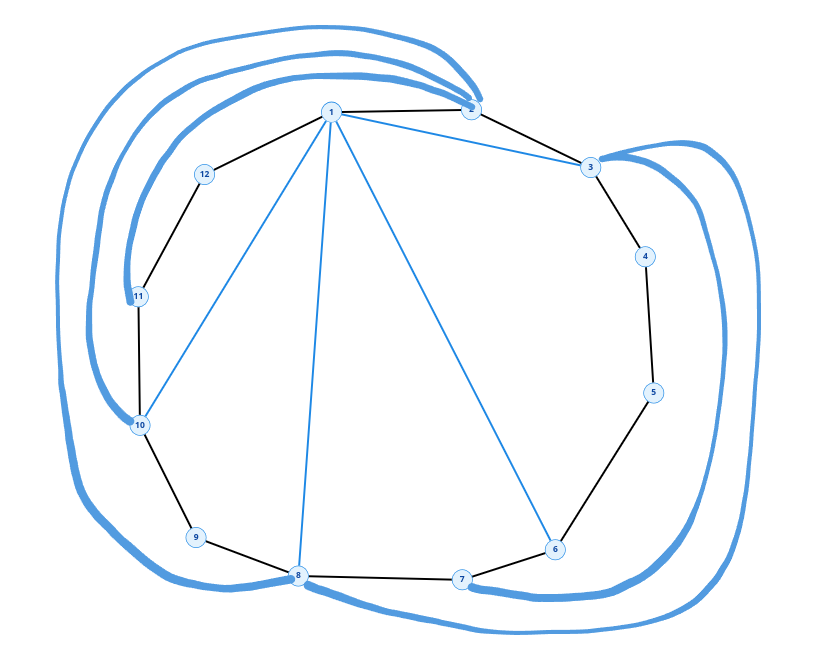
\includegraphics[width=0.7\linewidth]{images/4/plan1.png}
    \caption*{Планарный сурграф}
\end{figure}

\noindent
Удалим из $\psi_G$ все ребра вошедшие в $\psi_1$ и $\psi_{10}$, получим: \\
$\psi_{3} = \{u_{3\ 9}\}$\\
$\psi_{4} = \{u_{4\ 10}\}$\\
$\psi_{5} = \{u_{3\ 11},u_{3\ 9}\}$\\
$\psi_{6} = \{u_{3\ 11},u_{4\ 10}\}$\\
$\psi_{7} = \{u_{4\ 12},u_{4\ 10}\}$\\
$\psi_{8} = \{u_{4\ 12},u_{5\ 12}\}$\\
$\psi_{9} = \{u_{2\ 6}\}$\\
$\psi_{11} = \{u_{3\ 9}\}$\\
$\psi_{12} = \{u_{4\ 10}\}$\\
$\psi_{13} = \{u_{3\ 11},u_{3\ 9}\}$\\
$\psi_{14} = \{u_{3\ 11},u_{4\ 10}\}$\\
$\psi_{15} = \{u_{2\ 6}\}$\\
$\psi_{16} = \{u_{2\ 6}\}$\\
$\psi_{18} = \{u_{2\ 6}\}$\\
$\psi_{20} = \{u_{3\ 9}\}$\\
$\psi_{21} = \{u_{4\ 10}\}$\\
$\psi_{22} = \{u_{2\ 6}\}$\\
Объединим одинаковые множества: \\
$\psi_{3} = \{u_{3\ 9}\}$\\
$\psi_{4} = \{u_{4\ 10}\}$\\
$\psi_{5} = \{u_{3\ 11},u_{3\ 9}\}$\\
$\psi_{6} = \{u_{3\ 11},u_{4\ 10}\}$\\
$\psi_{7} = \{u_{4\ 12},u_{4\ 10}\}$\\
$\psi_{8} = \{u_{4\ 12},u_{5\ 12}\}$\\
$\psi_{9} = \{u_{2\ 6}\}$\\

\newpage
\noindent
Выделим максимальный двудольный подграф. Для каждой пары множеств вычислим значение критерия $\alpha_{\gamma\beta} = |\psi_\gamma| + |\psi_\beta| - |\psi_\gamma \cap \psi_\beta|$:\\
$\alpha_{3\ 4} = 1 + 1 - 0  = 2$ \\
$\alpha_{3\ 5} = 1 + 2 - 1 = 2$ \\
$\alpha_{3\ 6} = 1 + 2 - 0 = 3$ \\
$\alpha_{3\ 7} = 1 + 2 - 0 = 3$ \\
$\alpha_{3\ 8} = 1 + 2 - 0 = 3$ \\
$\alpha_{3\ 9} = 1 + 1 - 0 = 2$ \\
$\alpha_{4\ 5} = 1 + 2 - 0 = 3$ \\
$\alpha_{4\ 6} = 1 + 2 - 1 = 2$ \\
$\alpha_{4\ 7} = 1 + 2 - 1 = 2$ \\
$\alpha_{4\ 8} = 1 + 2 - 0 = 3$ \\
$\alpha_{4\ 9} = 1 + 1 - 0 = 2$ \\
$\alpha_{5\ 6} = 2 + 2 - 1 = 3$ \\
$\alpha_{5\ 7} = 2 + 2 - 0 = 4$ \\
$\alpha_{5\ 8} = 2 + 2 - 0 = 4$ \\
$\alpha_{5\ 9} = 2 + 1 - 0 = 3$ \\
$\alpha_{6\ 7} = 2 + 2 - 1 = 3$ \\
$\alpha_{6\ 8} = 2 + 2 - 0 = 4$ \\
$\alpha_{6\ 9} = 2 + 1 - 0 = 3$ \\
$\alpha_{7\ 8} = 2 + 2 - 1 = 3$ \\
$\alpha_{7\ 9} = 2 + 1 - 0 = 3$ \\
$\alpha_{8\ 9} = 2 + 1 - 0 = 3$ \\
$max(\alpha_{\gamma\delta}) = \alpha_{5\ 7} = \alpha_{5\ 8} = \alpha_{6\ 8} = 4$ дают пары множеств $\{\psi_{5},\psi_{7}\}$, $\{\psi_{5},\psi_{8}\}$ и $\{\psi_{6},\psi_{8}\}$
Возьмем множества $\psi_{5} = \{u_{3\ 11},u_{3\ 9}\}$ и $\psi_{7} = \{u_{4\ 12}, u_{4\ 10}\}$ \\
В сурграфе $H$, ребра, вошедшие в $\psi_5$, проведем внутри гамильтонова цикла, а в $\psi_{7}$ - вне его 
\begin{figure}[H]
    \centering
    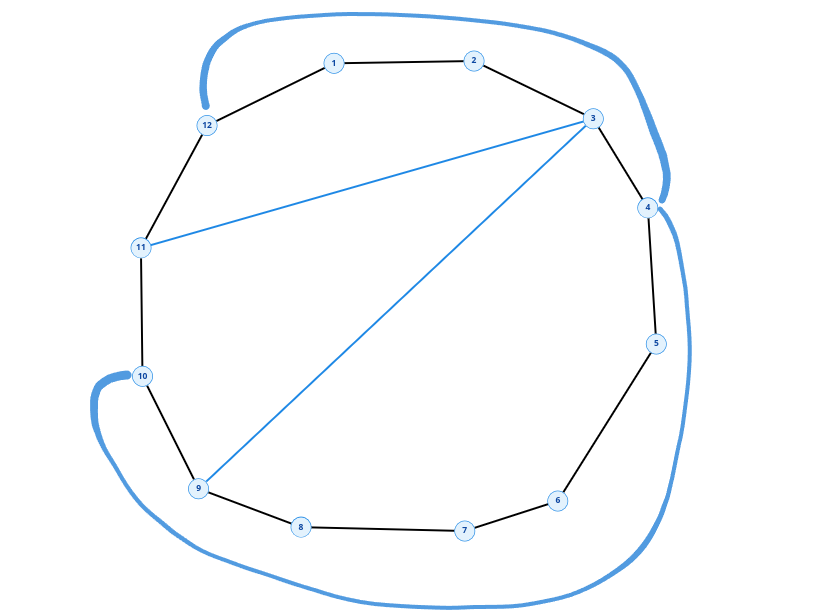
\includegraphics[width=0.7\linewidth]{images/4/plan2.png}
    \caption*{Планарный сурграф}
\end{figure}

\newpage
\noindent
Удалим из $\psi_G$ все ребра вошедшие в $\psi_5$ и $\psi_{7}$, получим: \\
$\psi_{8} = \{u_{5\ 12}\}$\\
$\psi_{9} = \{u_{2\ 6}\}$\\

\noindent
Остались ребра $u_{5\ 12}$ и $u_{2\ 6}$. Проведем их
\begin{figure}[H]
    \centering
    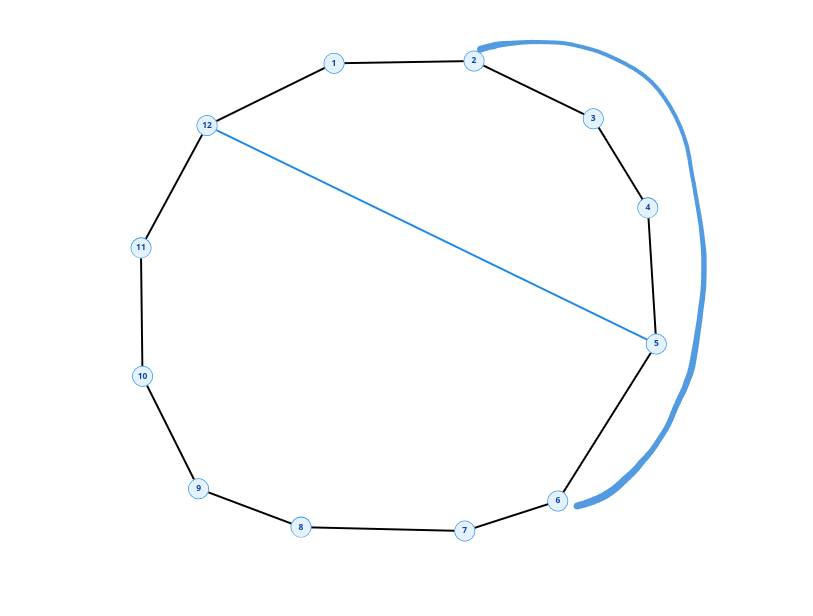
\includegraphics[width=0.7\linewidth]{images/4/plan3.png}
    \caption*{Планарный сурграф}
\end{figure}

\noindent
Итого реализовано $15+12=27$ ребер. Толщина графа $m=3$.

\end{document}